\documentclass[a4paper]{article}
\usepackage[left=2cm, right=2cm,bottom=2cm]{geometry}
\usepackage{lipsum}
\usepackage{tikzpagenodes}
\usepackage{pgfplots}
\usepackage{tikz}
\usepackage{tikz-3dplot}
\usetikzlibrary{arrows,decorations.pathmorphing,backgrounds,positioning,fit,matrix}
\pgfplotsset{compat=1.8}
\usepackage{graphics} % for pdf, bitmapped graphics files
\usepackage{epsfig} % for postscript graphics files
\usepackage[colorlinks=true,citecolor=green]{hyperref}
\usepackage{cite}
\usepackage{amsmath,amssymb,amsfonts}
\usepackage{algorithmic}
\usepackage{graphicx}
\usepackage{url}
\usepackage{cite}
\usepackage{bm}
\usepackage{pbox}
\usepackage{siunitx,booktabs,etoolbox}
\usepackage{ulem}
\usepackage{titling}
\usepackage{float}
%\usepackage{pgf,tikz,pgfplots}
%\pgfplotsset{compat=1.15}
%\usepackage{mathrsfs}

\usetikzlibrary{arrows}

\def\BibTeX{{\rm B\kern-.05em{\sc i\kern-.025em b}\kern-.08em
		T\kern-.1667em\lower.7ex\hbox{E}\kern-.125emX}}
\title{Ex3: MRF, Deformable Models \& Geometric Priors}
\author{Xiao Hu, emails: \url{xiahaa@space.dtu.dk}}
\begin{document}
	\maketitle
	\thispagestyle{empty}
	\section{MRF Results}
	\begin{figure*}[htbp]
	\centering
	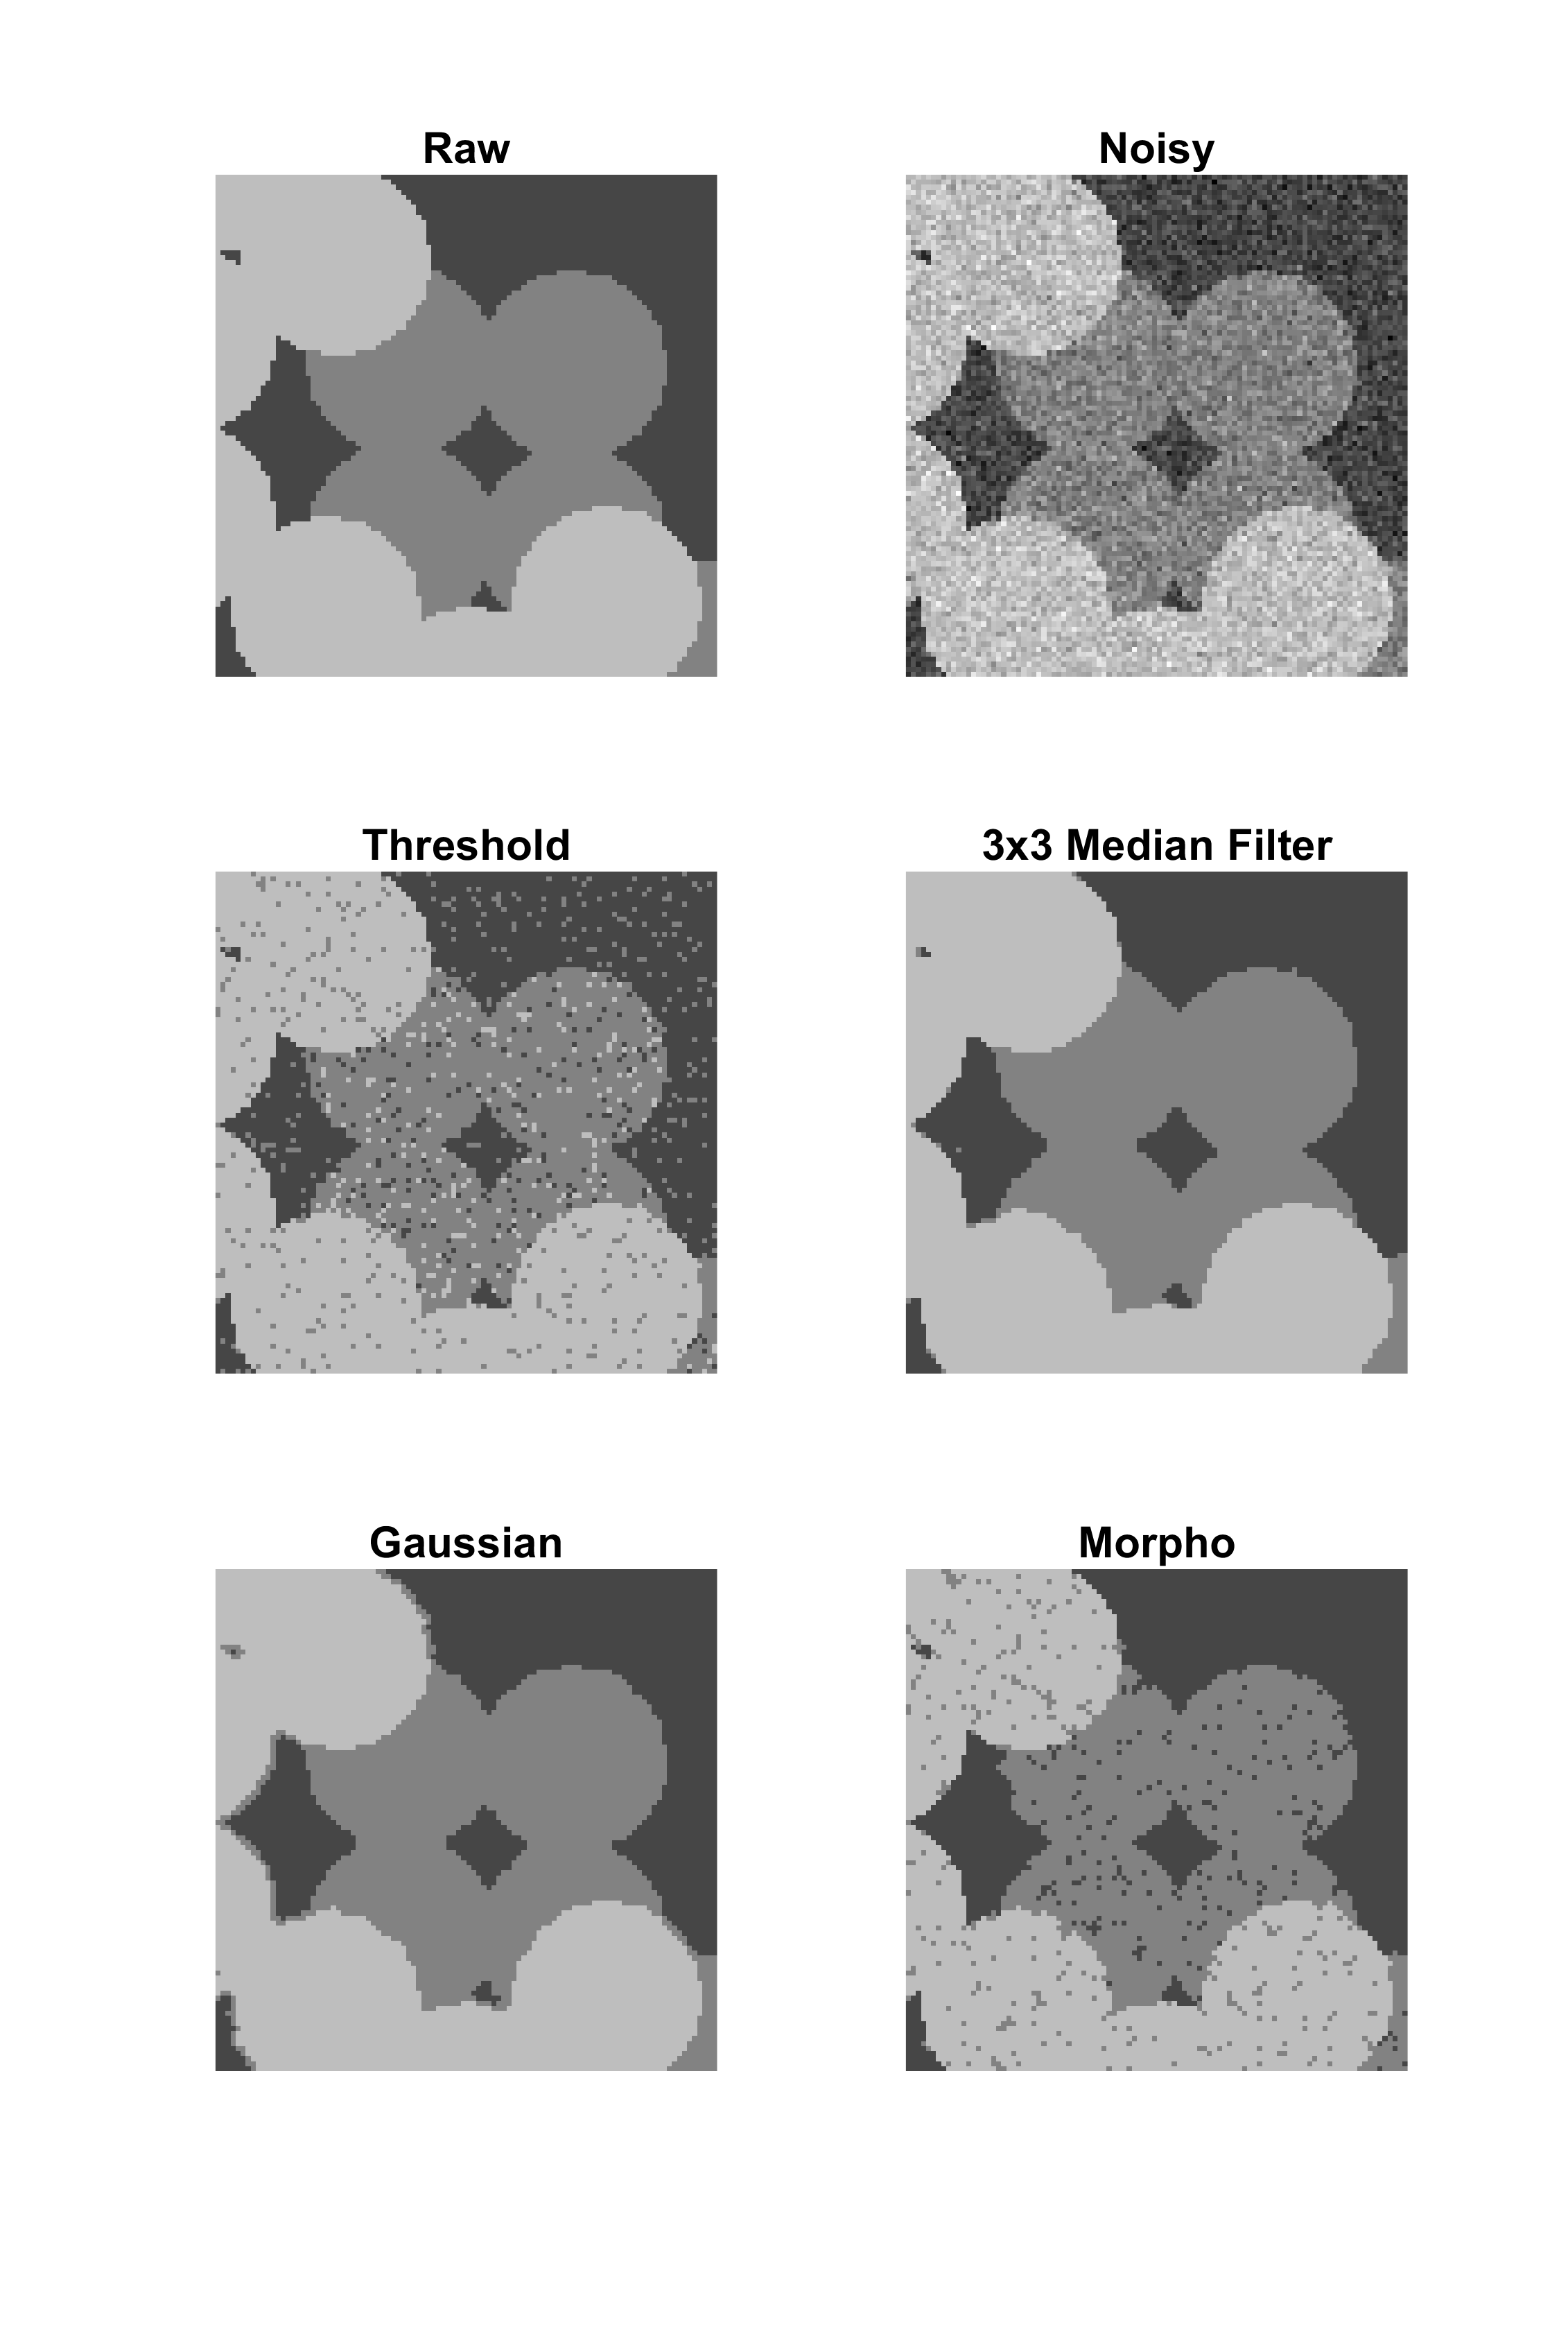
\includegraphics[width=0.54\textwidth]{./figures/res2.png}
	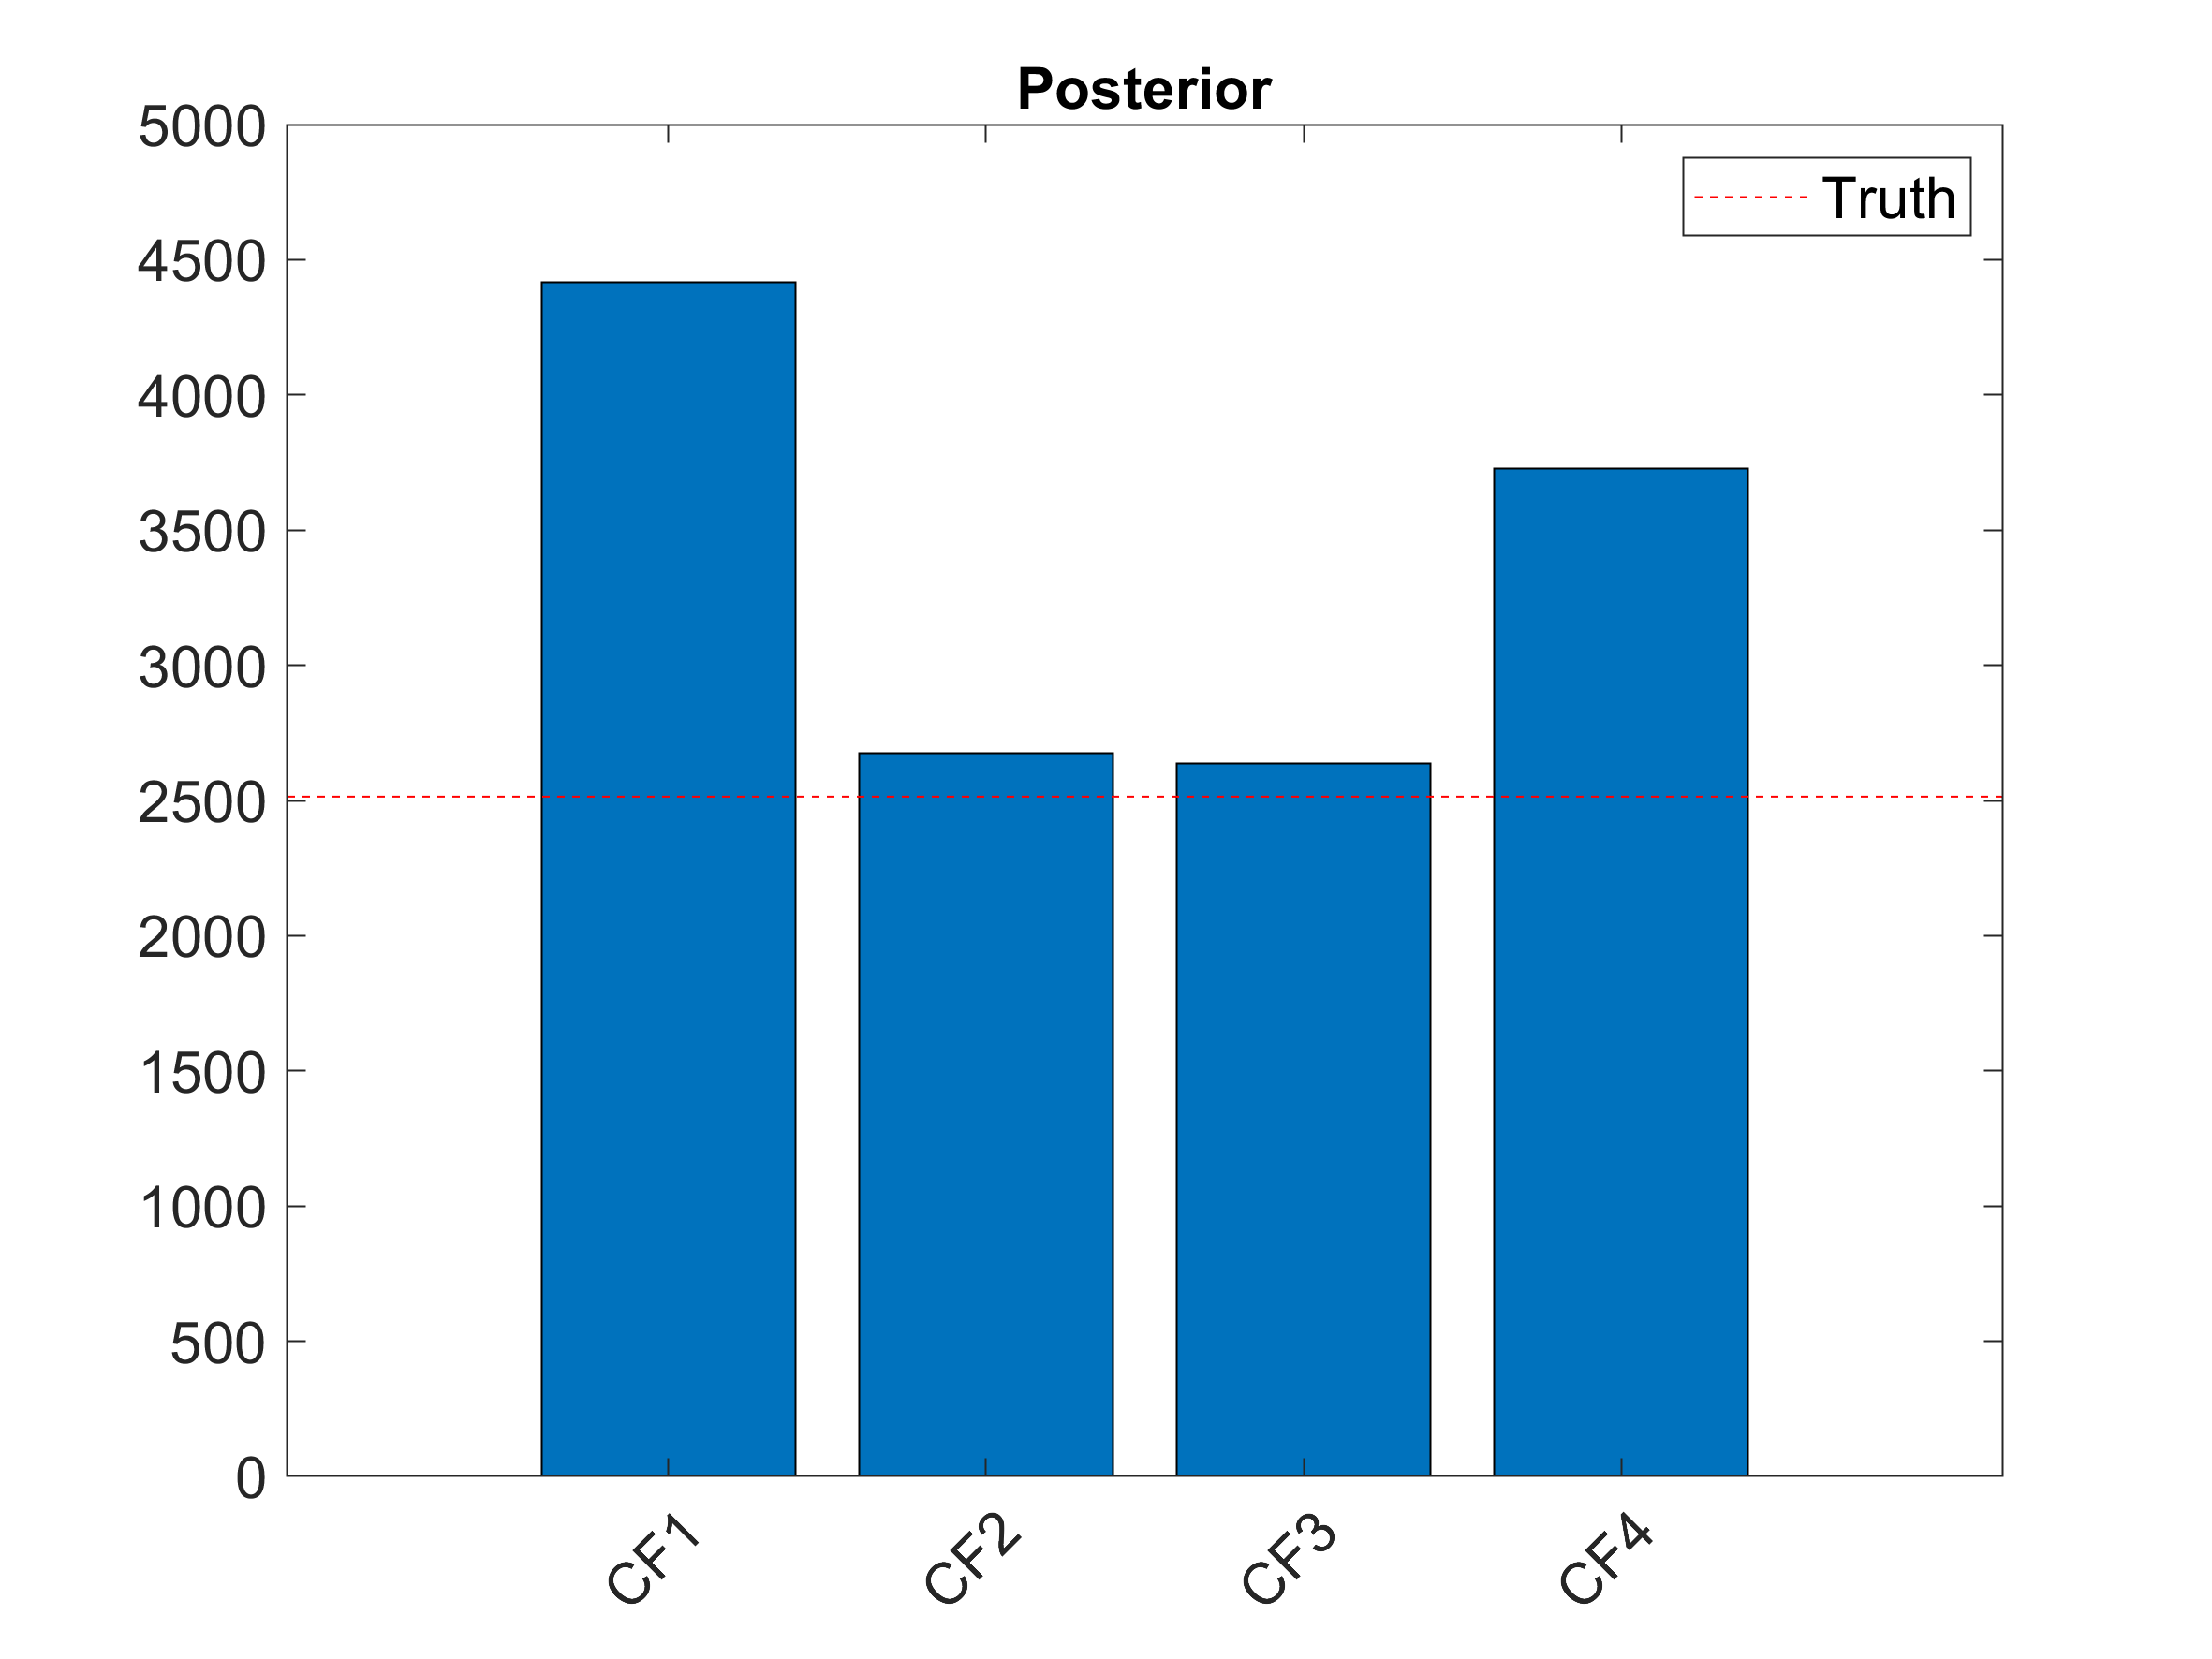
\includegraphics[width=0.45\textwidth]{./figures/res4.png}
	\caption{Left image shows the comparison of using four simple configurations. Visually speaking, the median filter based configuration can give us the best result. A guess would be that the added noise could be salty noise. Simple threshold cannot produce promising result. However, it can be improved by applying a Gaussian filter in advance. The cost to pay it that the edges may be destroyed to some extent. Right image shows the cost comparison: it is clear that the median filter and Gaussian filter give the most approximated results compared with ground truth.}
\end{figure*}

	\begin{figure}[htbp]
	\centering
	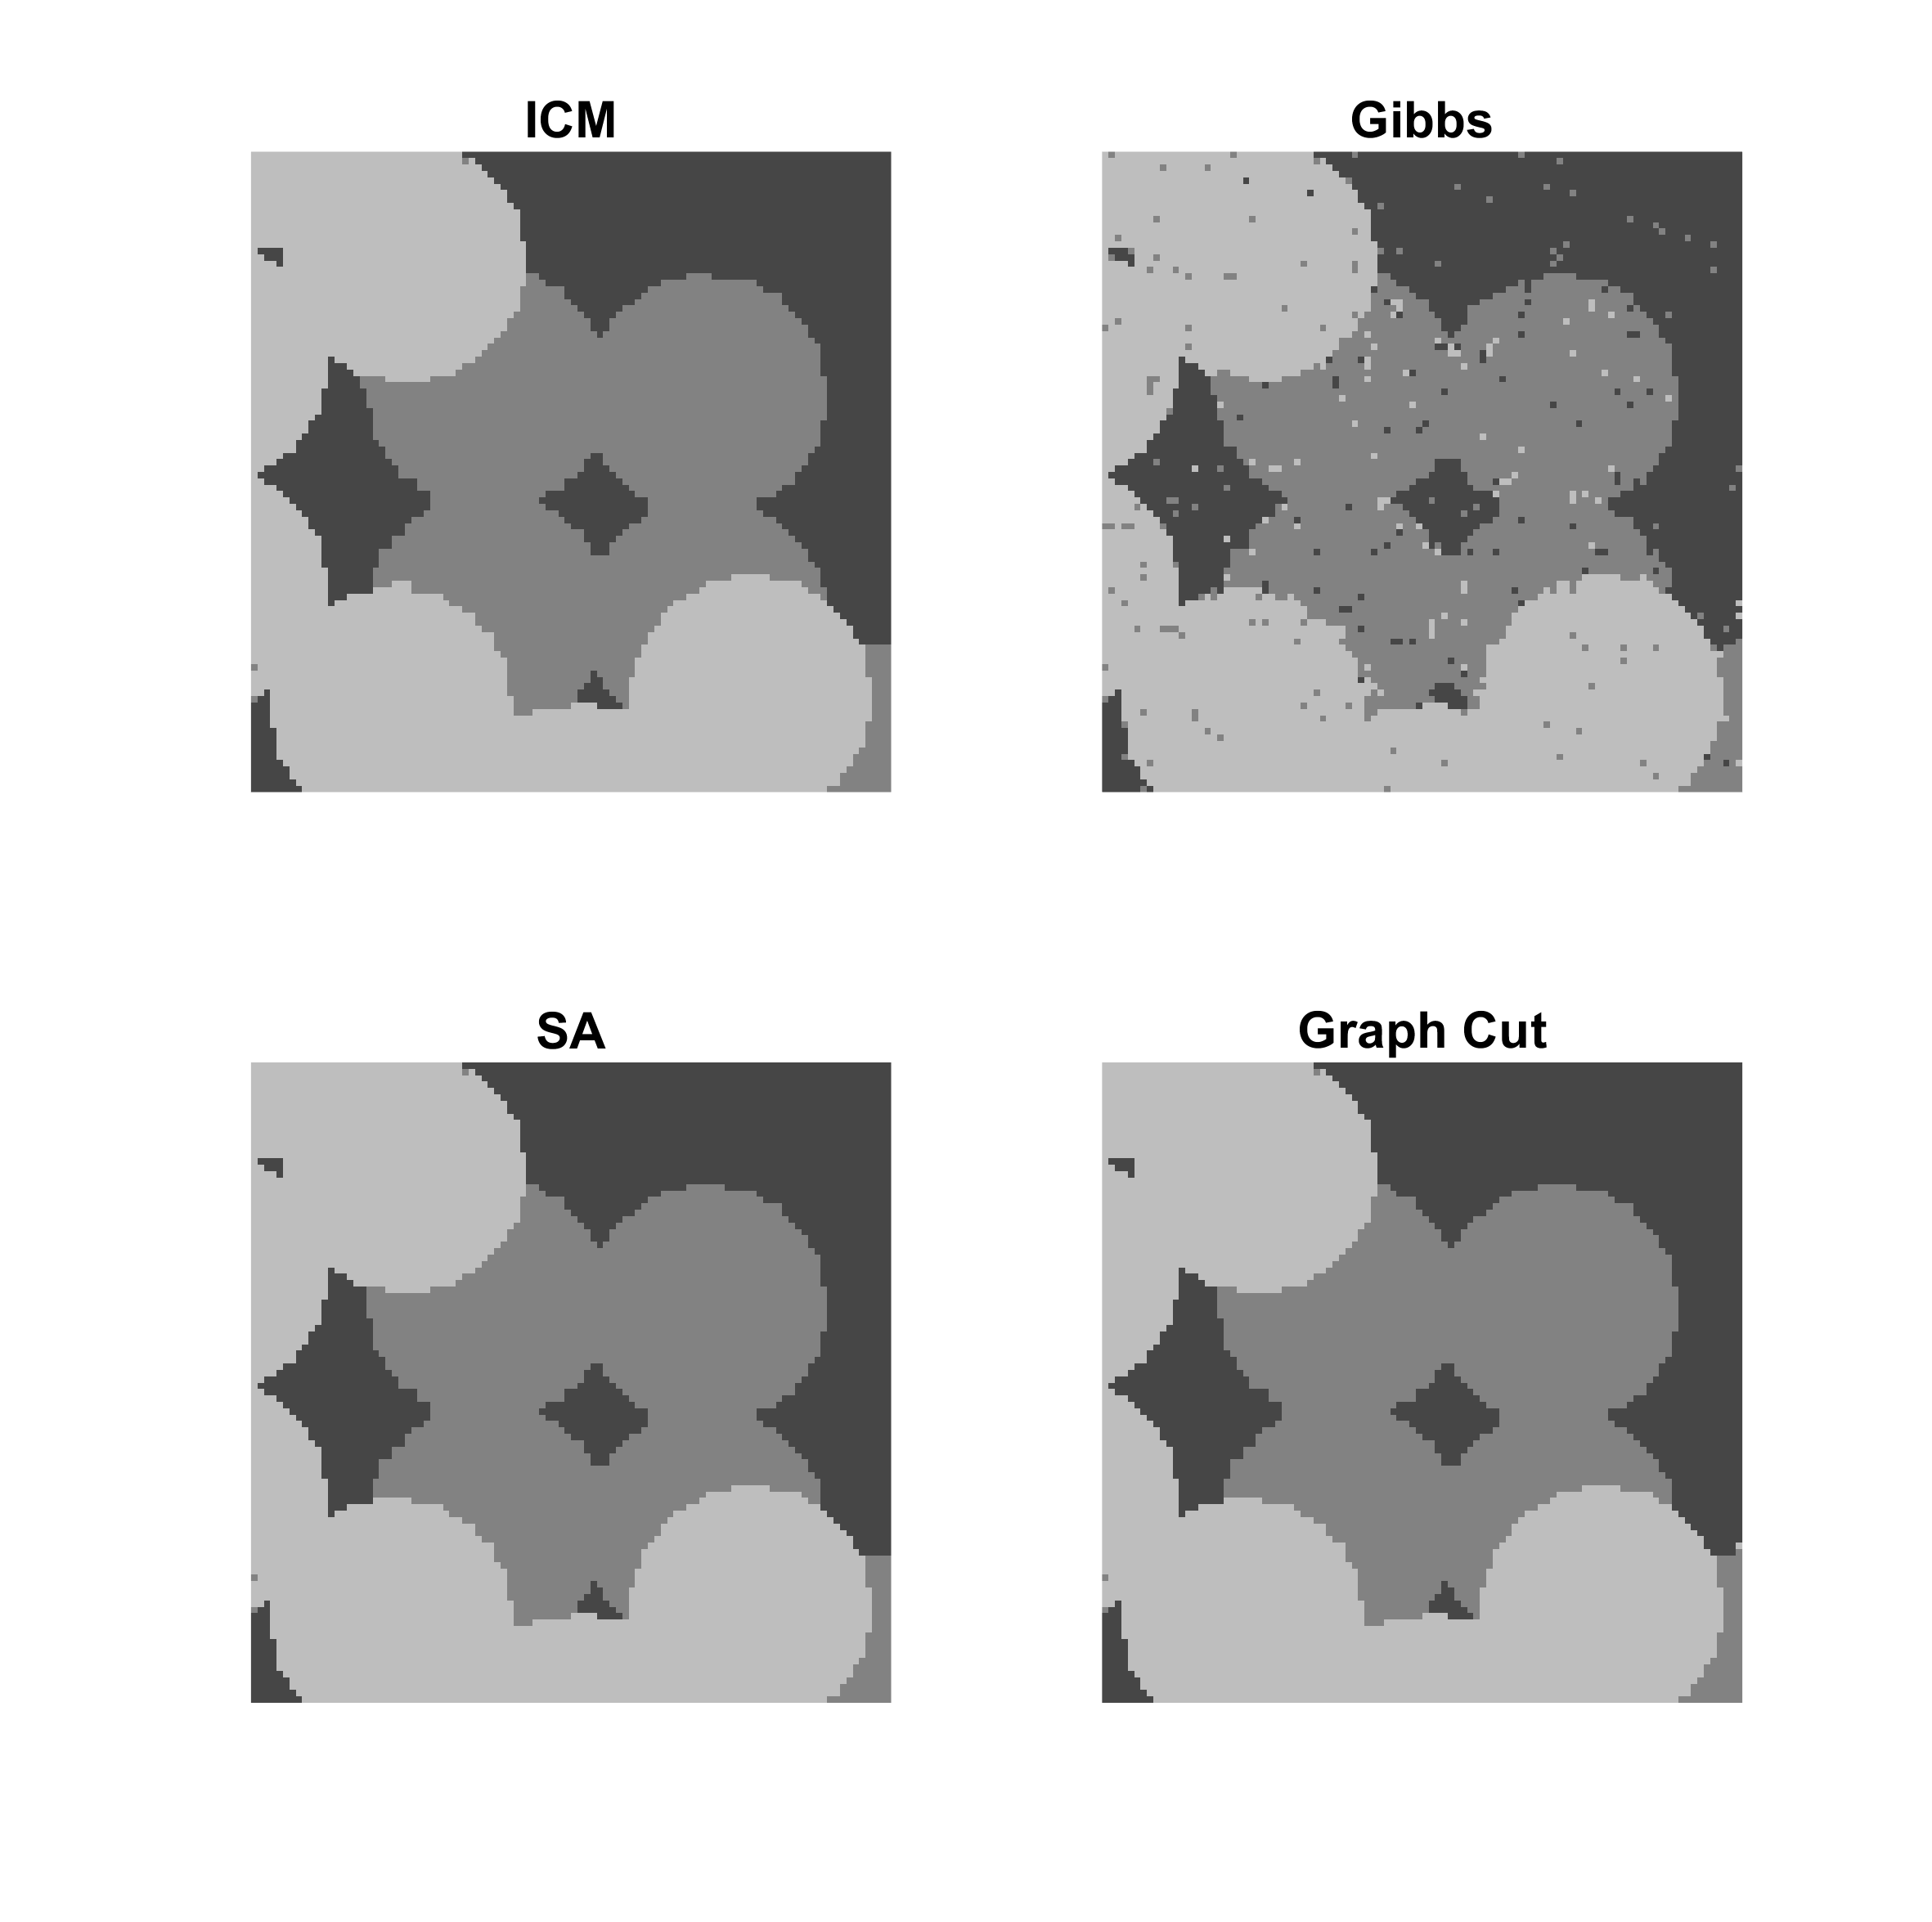
\includegraphics[width=0.6\textwidth]{./figures/cmp1.png}
	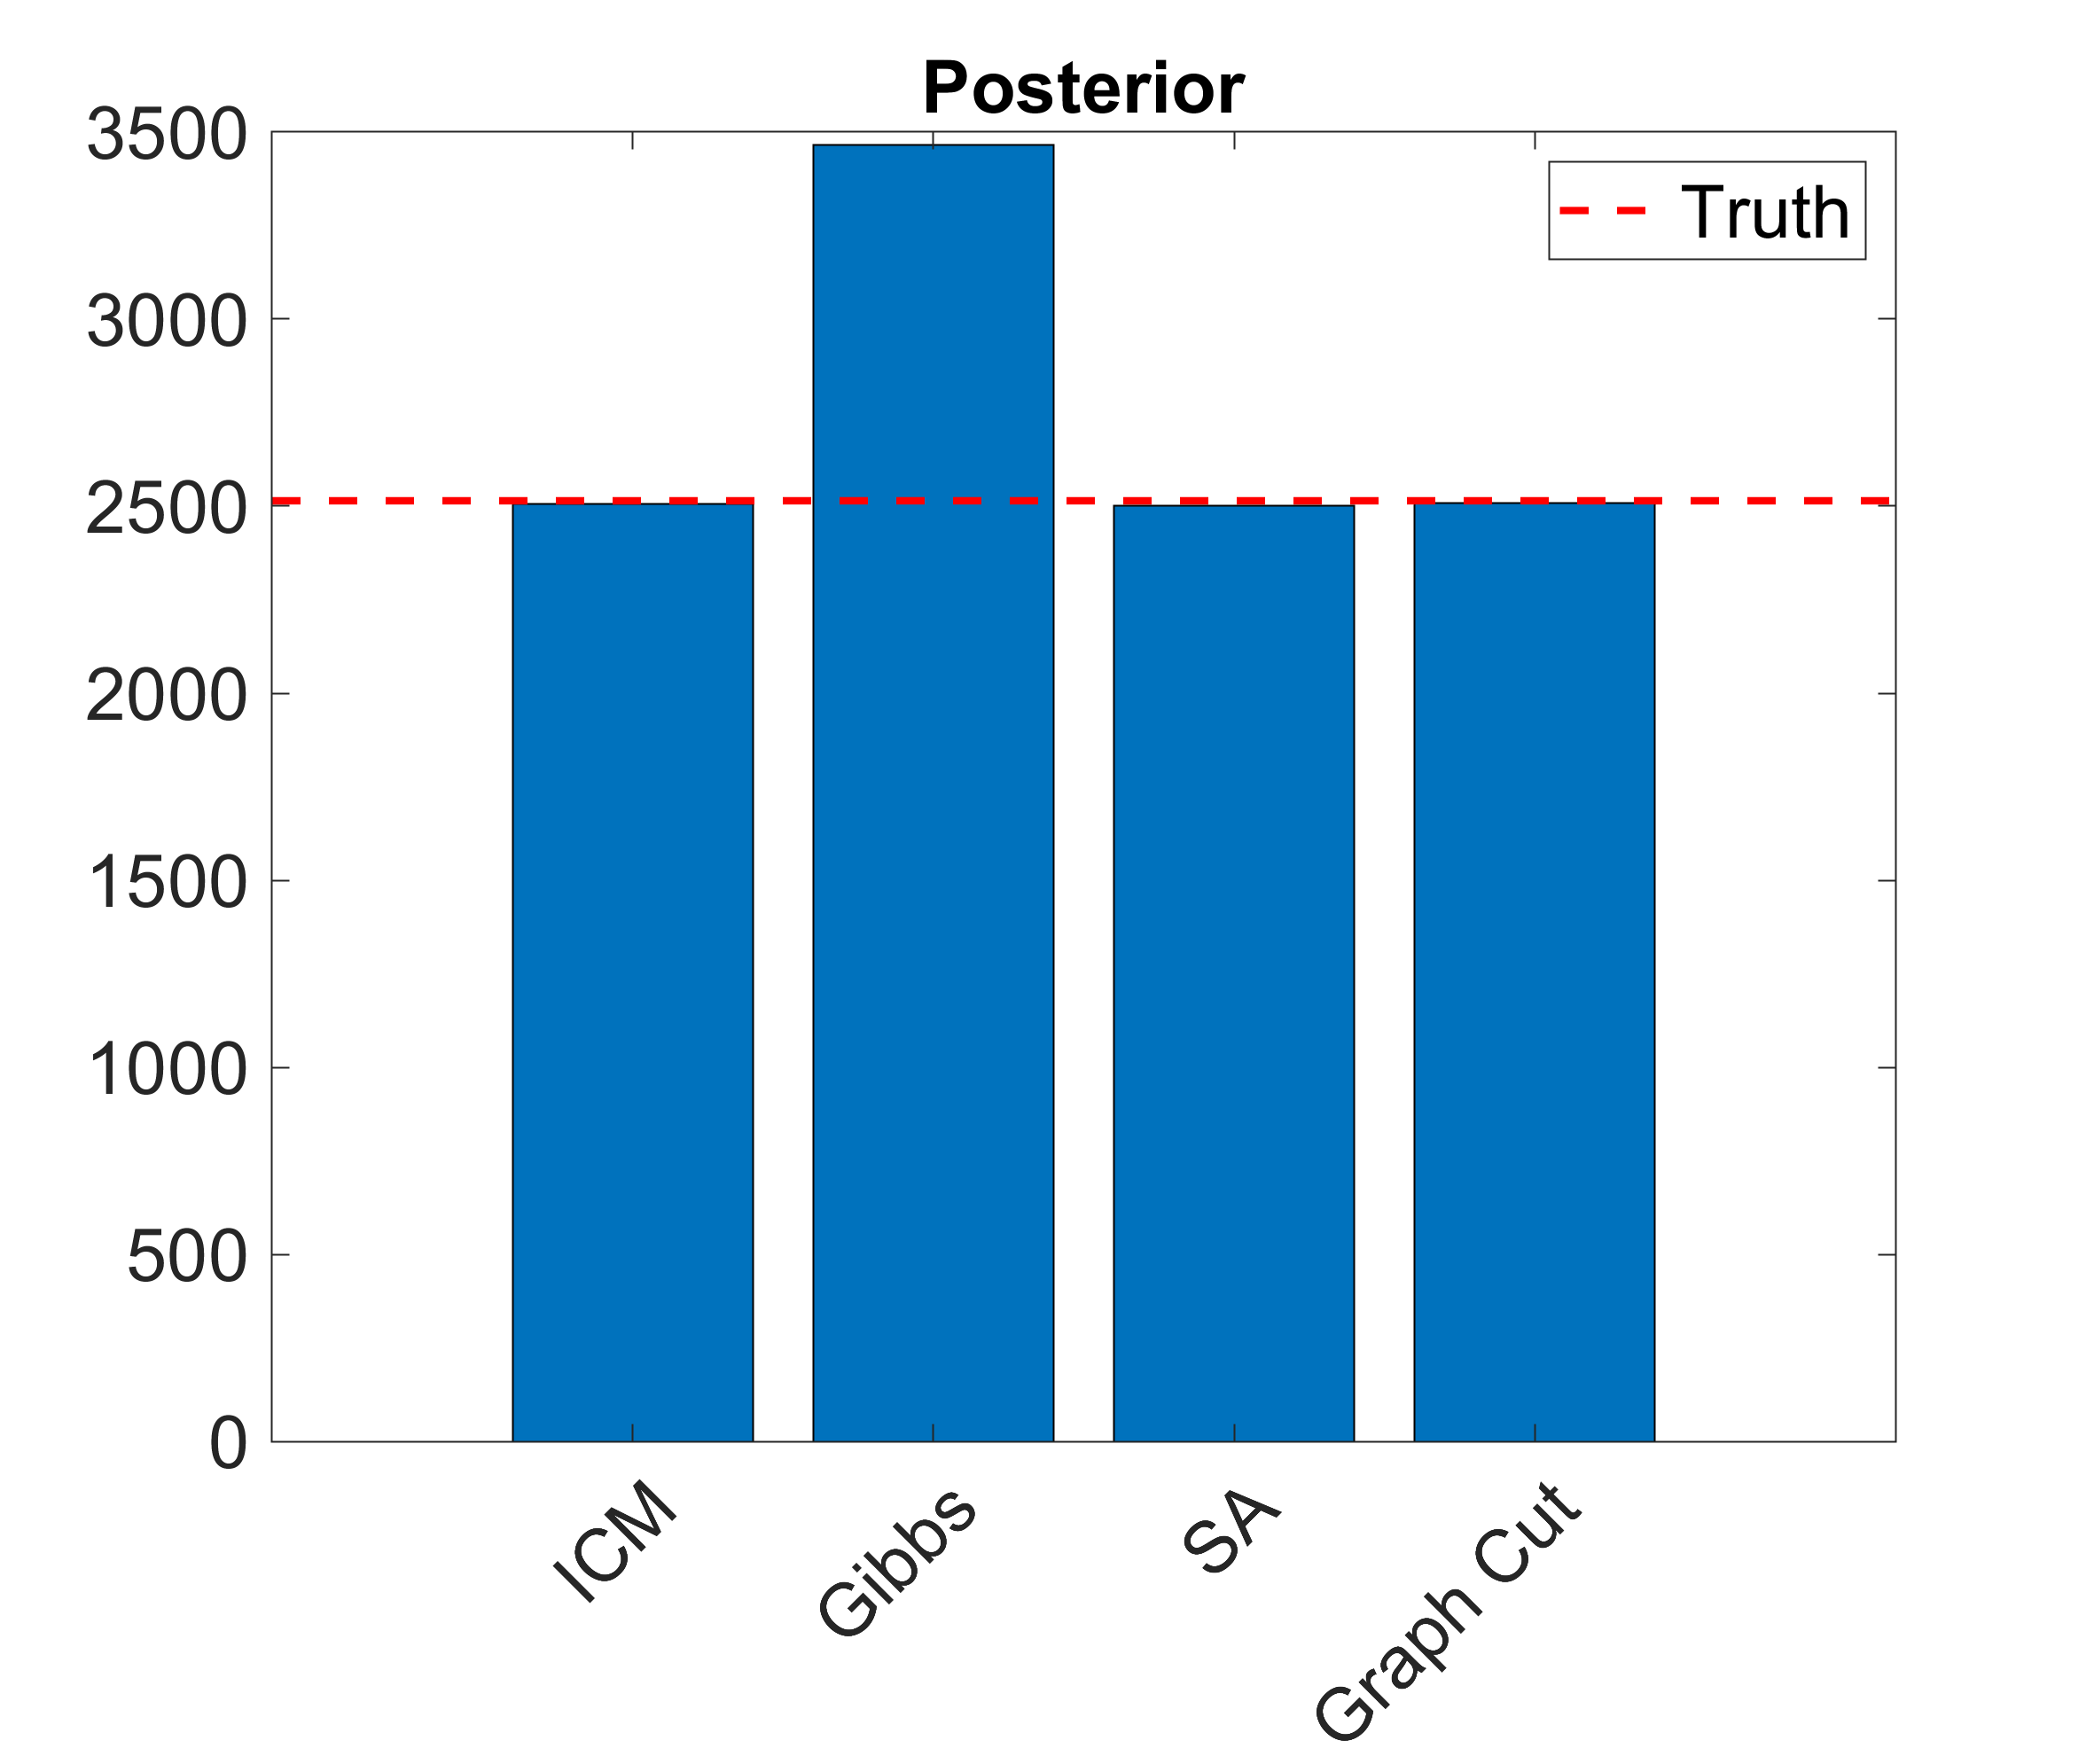
\includegraphics[width=0.38\textwidth]{./figures/cmp2.png}
	\caption{Comparison of using MRF with different optimization approaches. Visually speaking, ICM, Simulated Annealing and Graph Cut give better performance than Gibbs Sampling method. Right image shows the cost for the four optimization approaches. It is clear that ICM, SA and Graph Cut all achieves the ground truth. However, local optimization method like ICM cannot always guarantee to achieve the global minimum. SA, however, is probabilistic optimum. So with the iteration increasing, its probability of achieving global optimum will increase up to 1. Graph cut is a global optimal method for binary label segmentation.}
\end{figure}

	\begin{figure}[htbp]
	\centering
	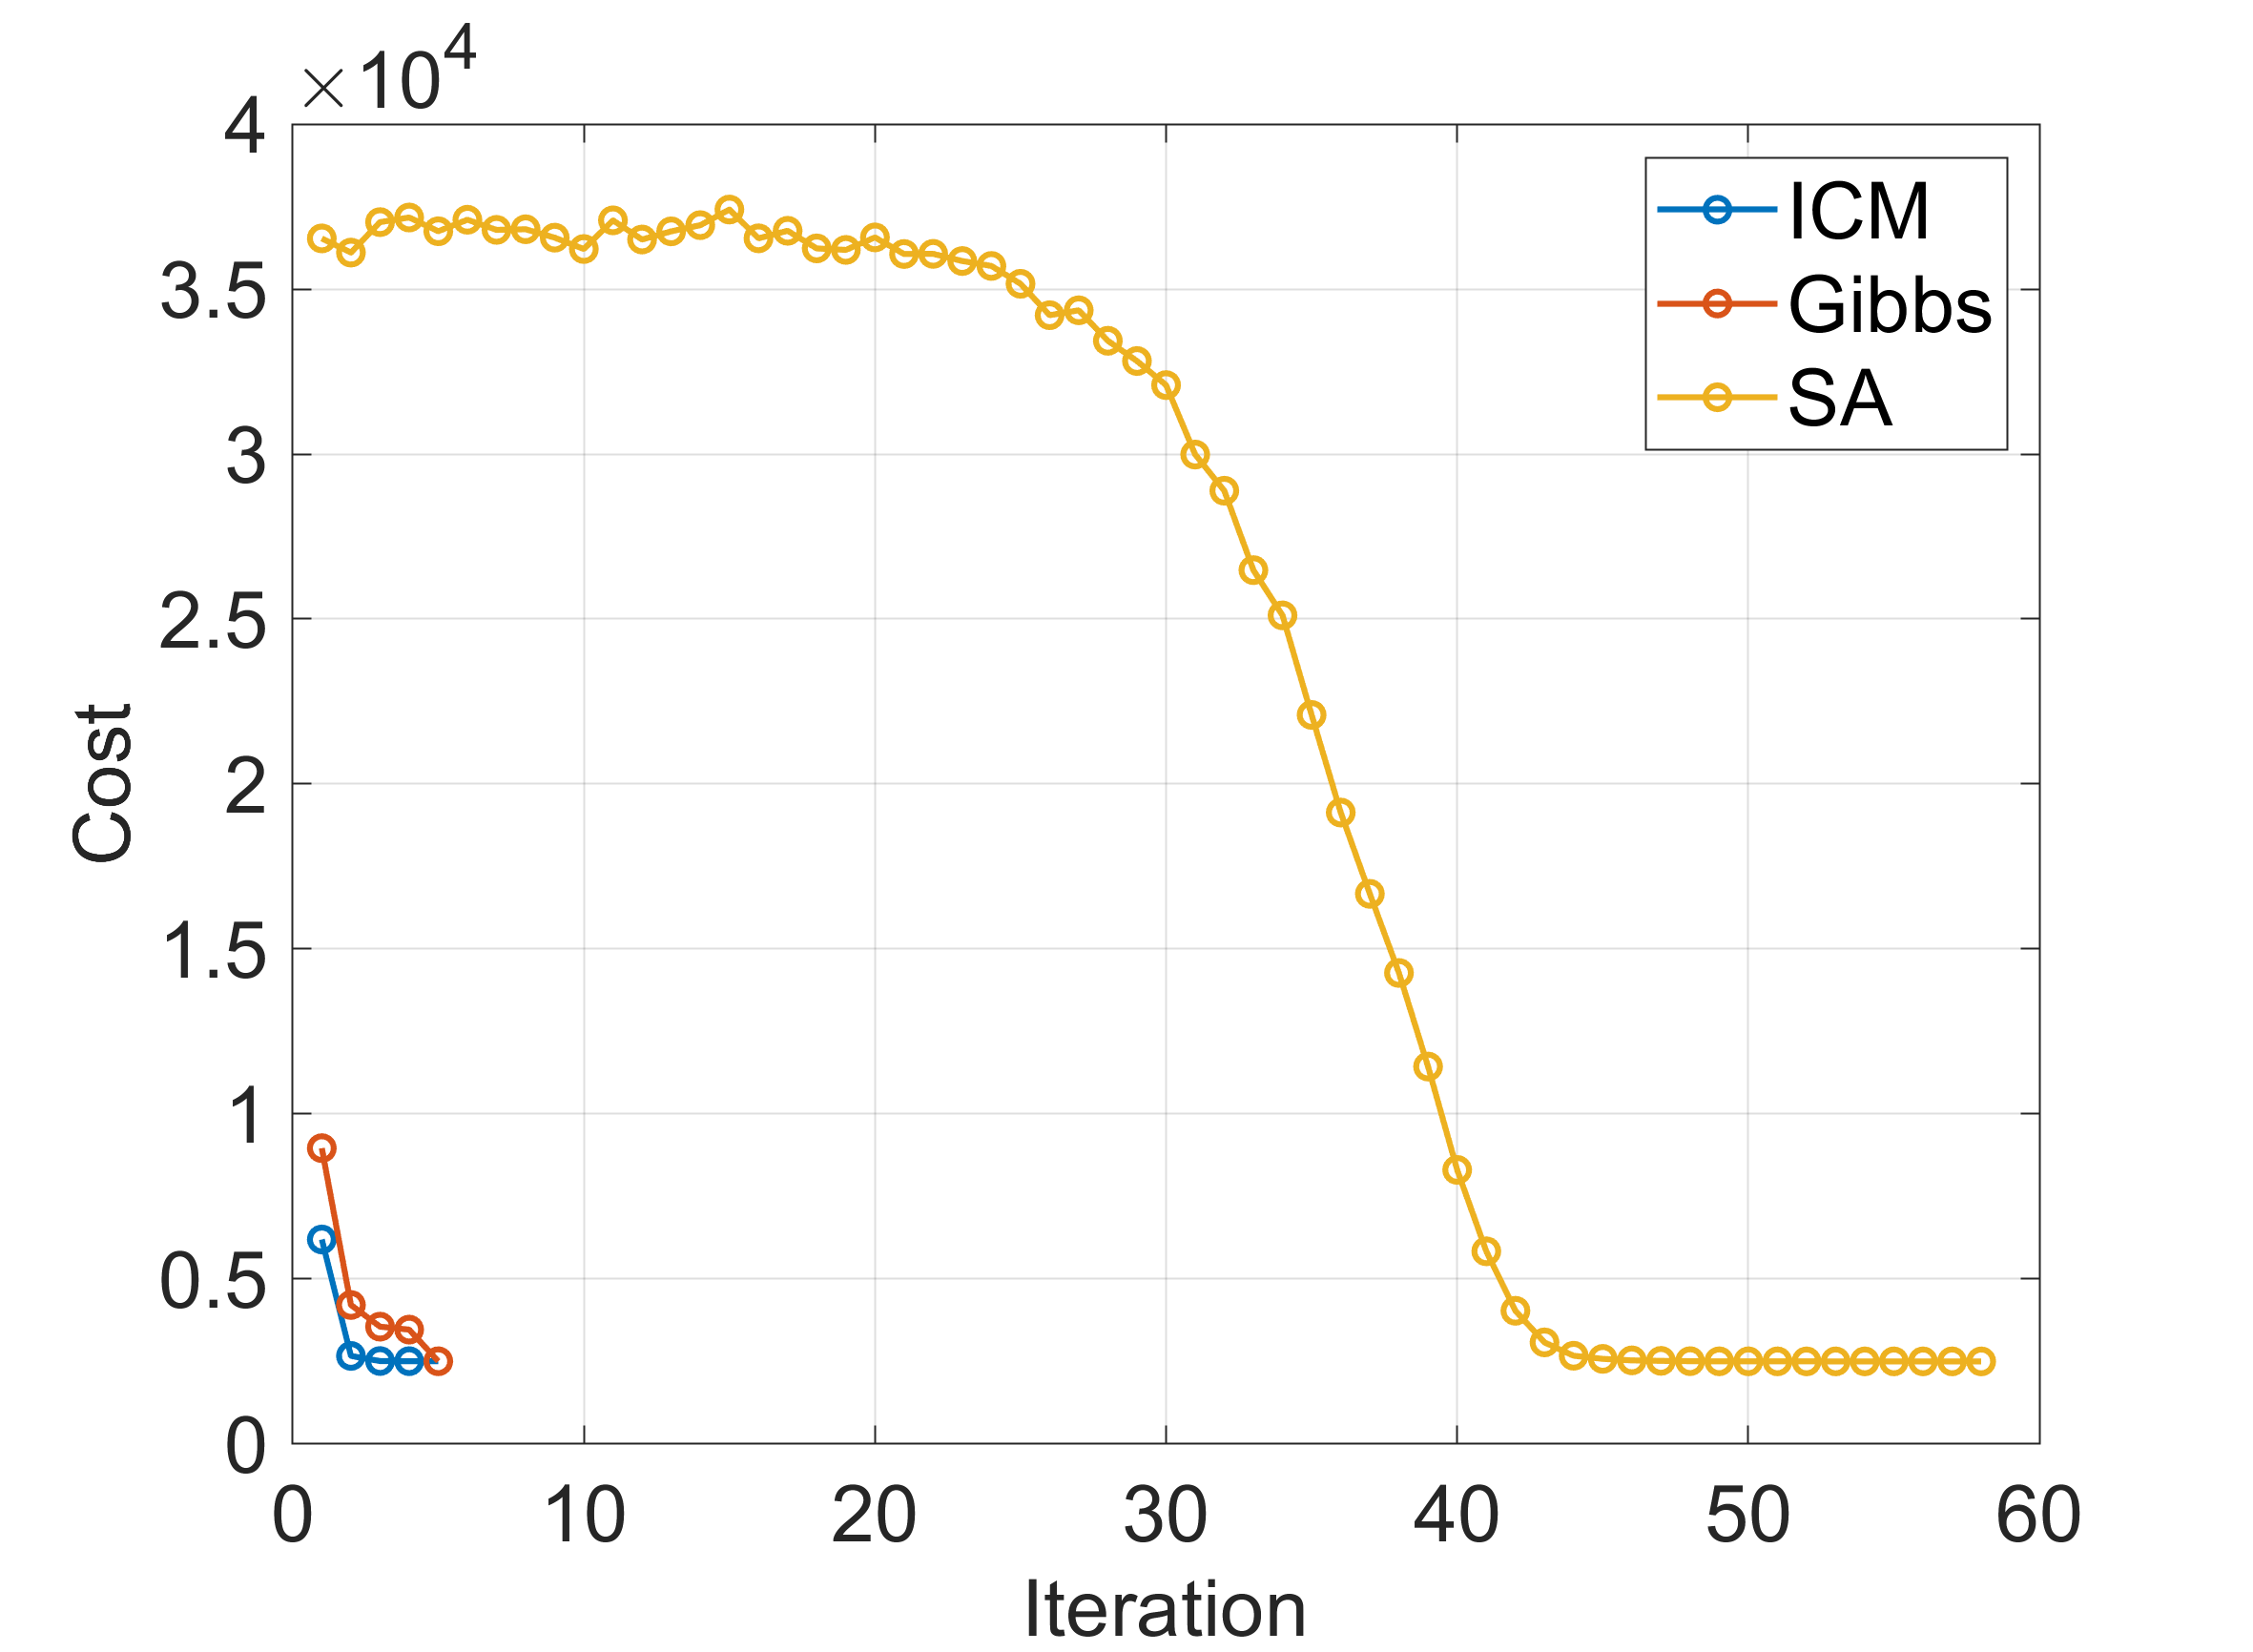
\includegraphics[width=0.5\textwidth]{./figures/cmp.png}
	\caption{Iteration comparison: SA will use more iteration to converge because it needs the temperature to be cooled down. Faster convergence can be achieved by make temperature cool down faster at a expense of increasing the possibility of being trapped in a local minimum. ICM and Gibbs sampling methods can converge rapidly compared with SA.}
\end{figure}

	\begin{figure}[htbp]
	\centering
	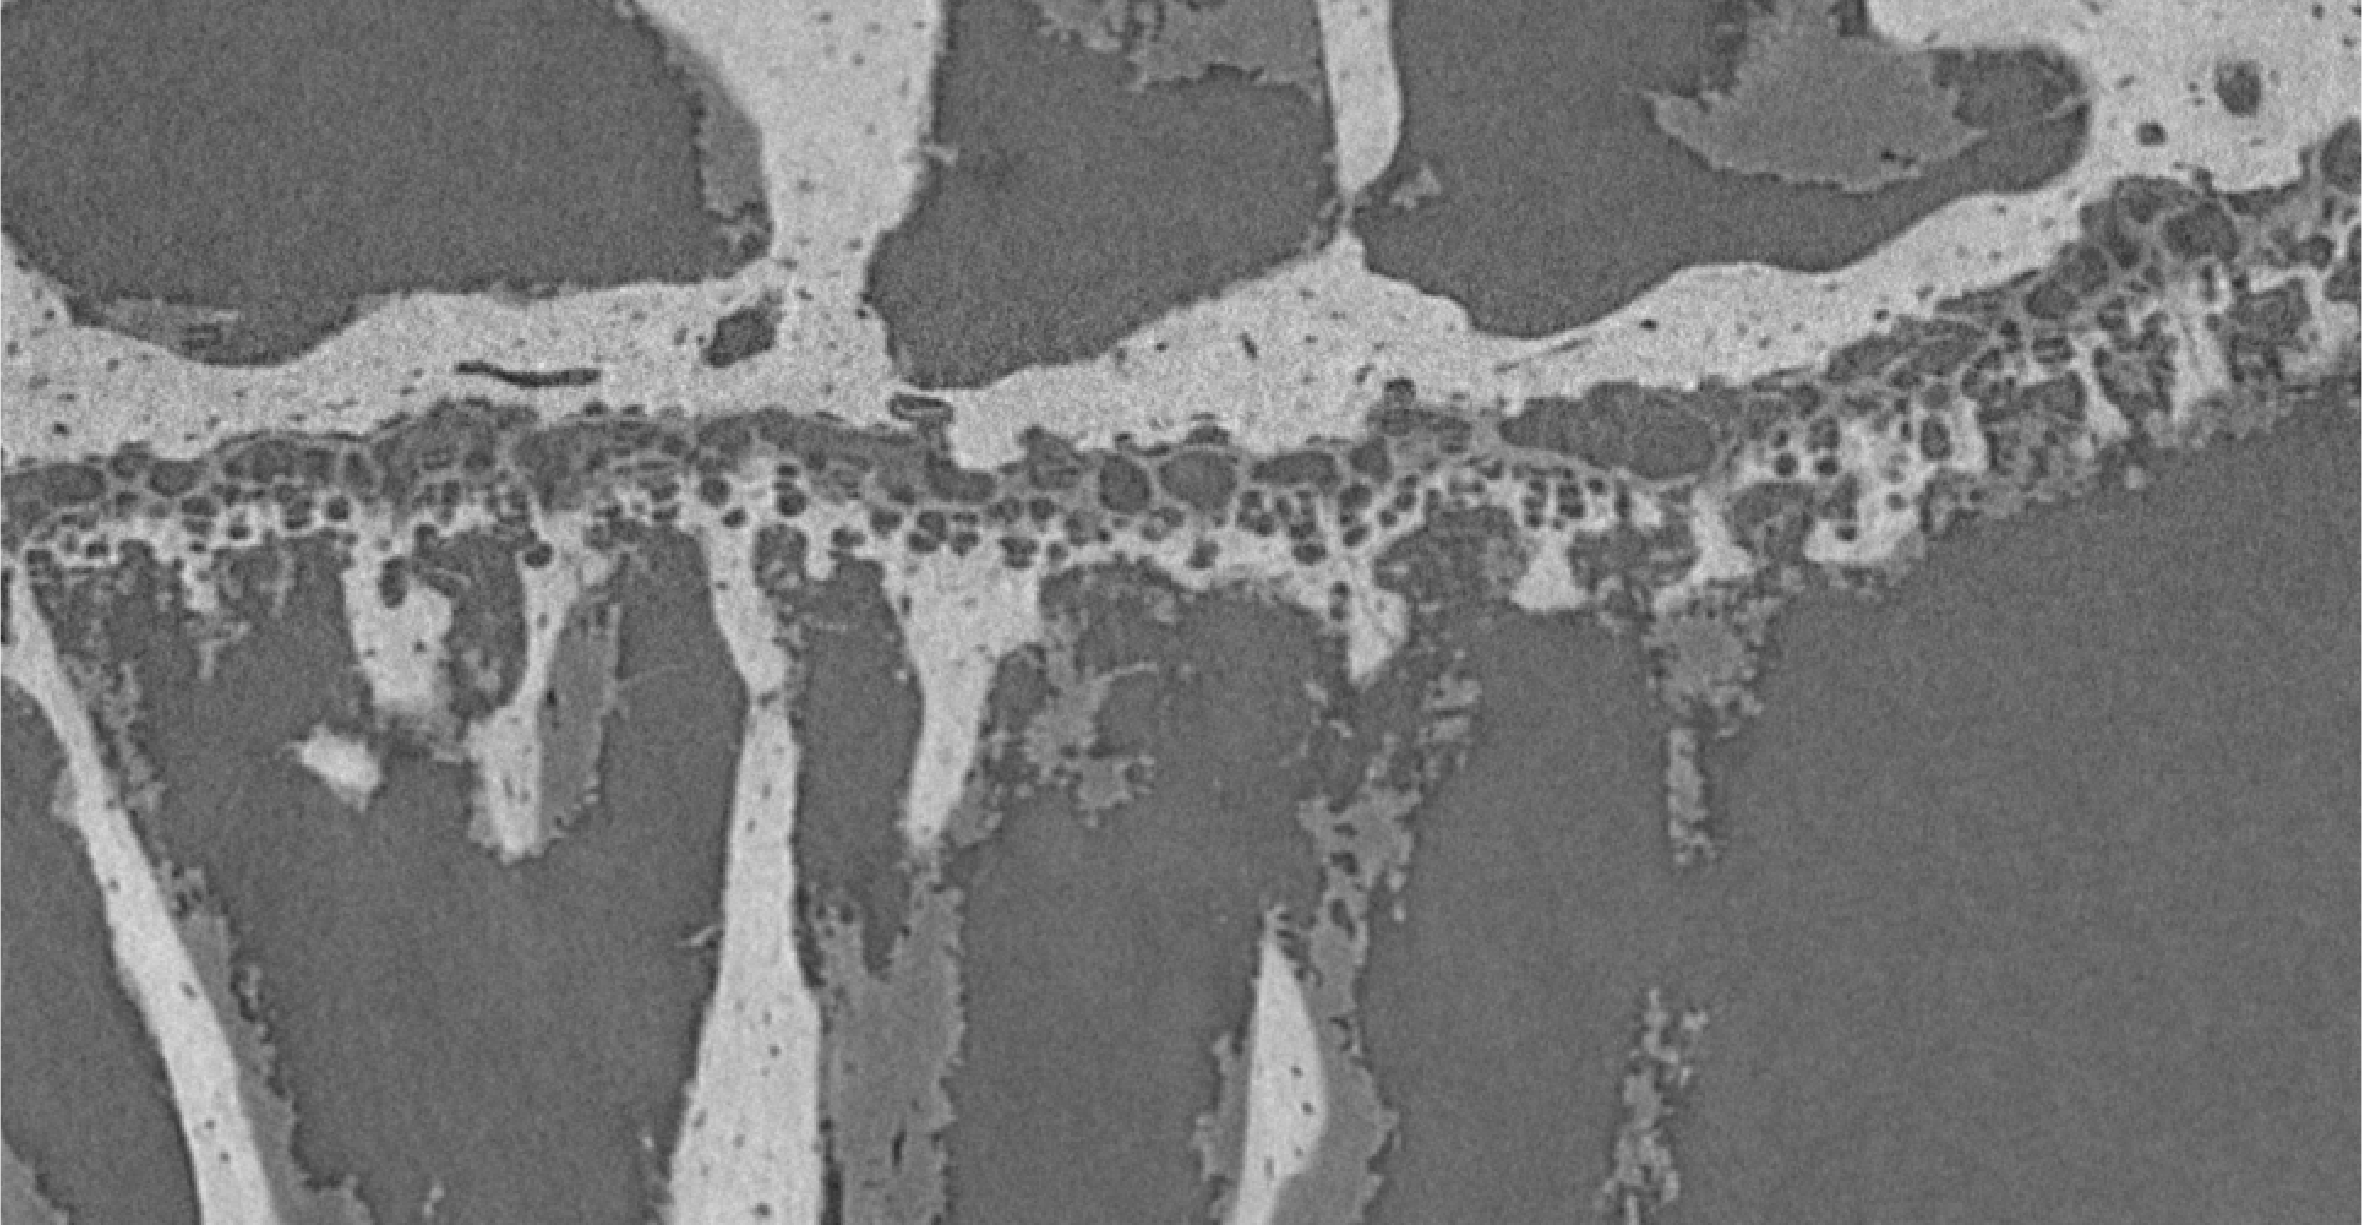
\includegraphics[width=0.5\textwidth]{./figures/assign2_raw.png}
	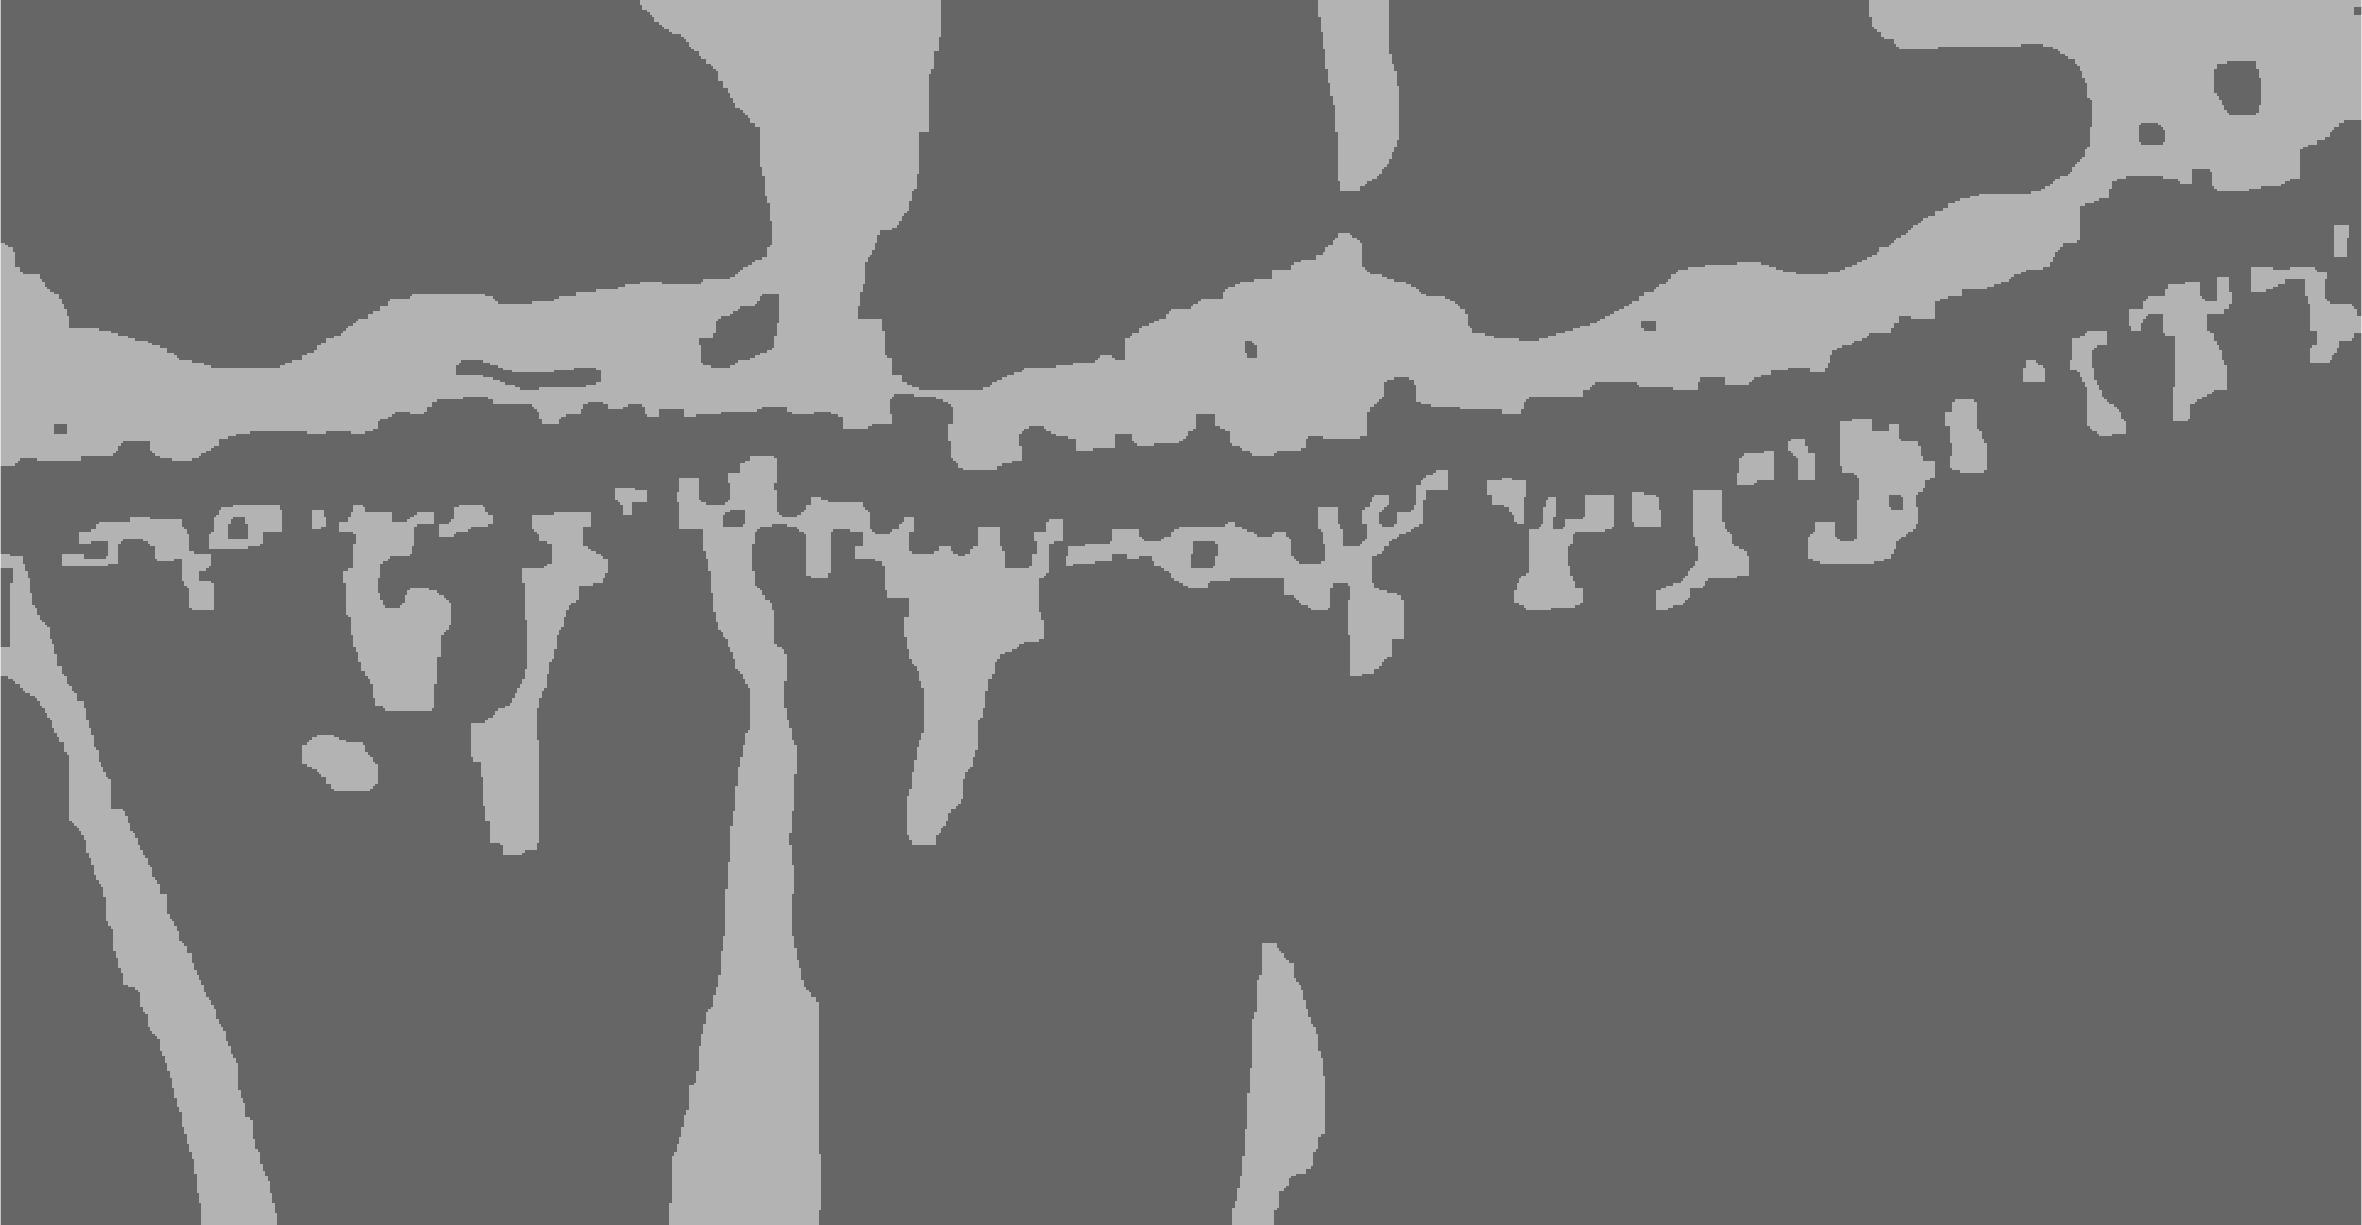
\includegraphics[width=0.5\textwidth]{./figures/assign2_seg.png}
	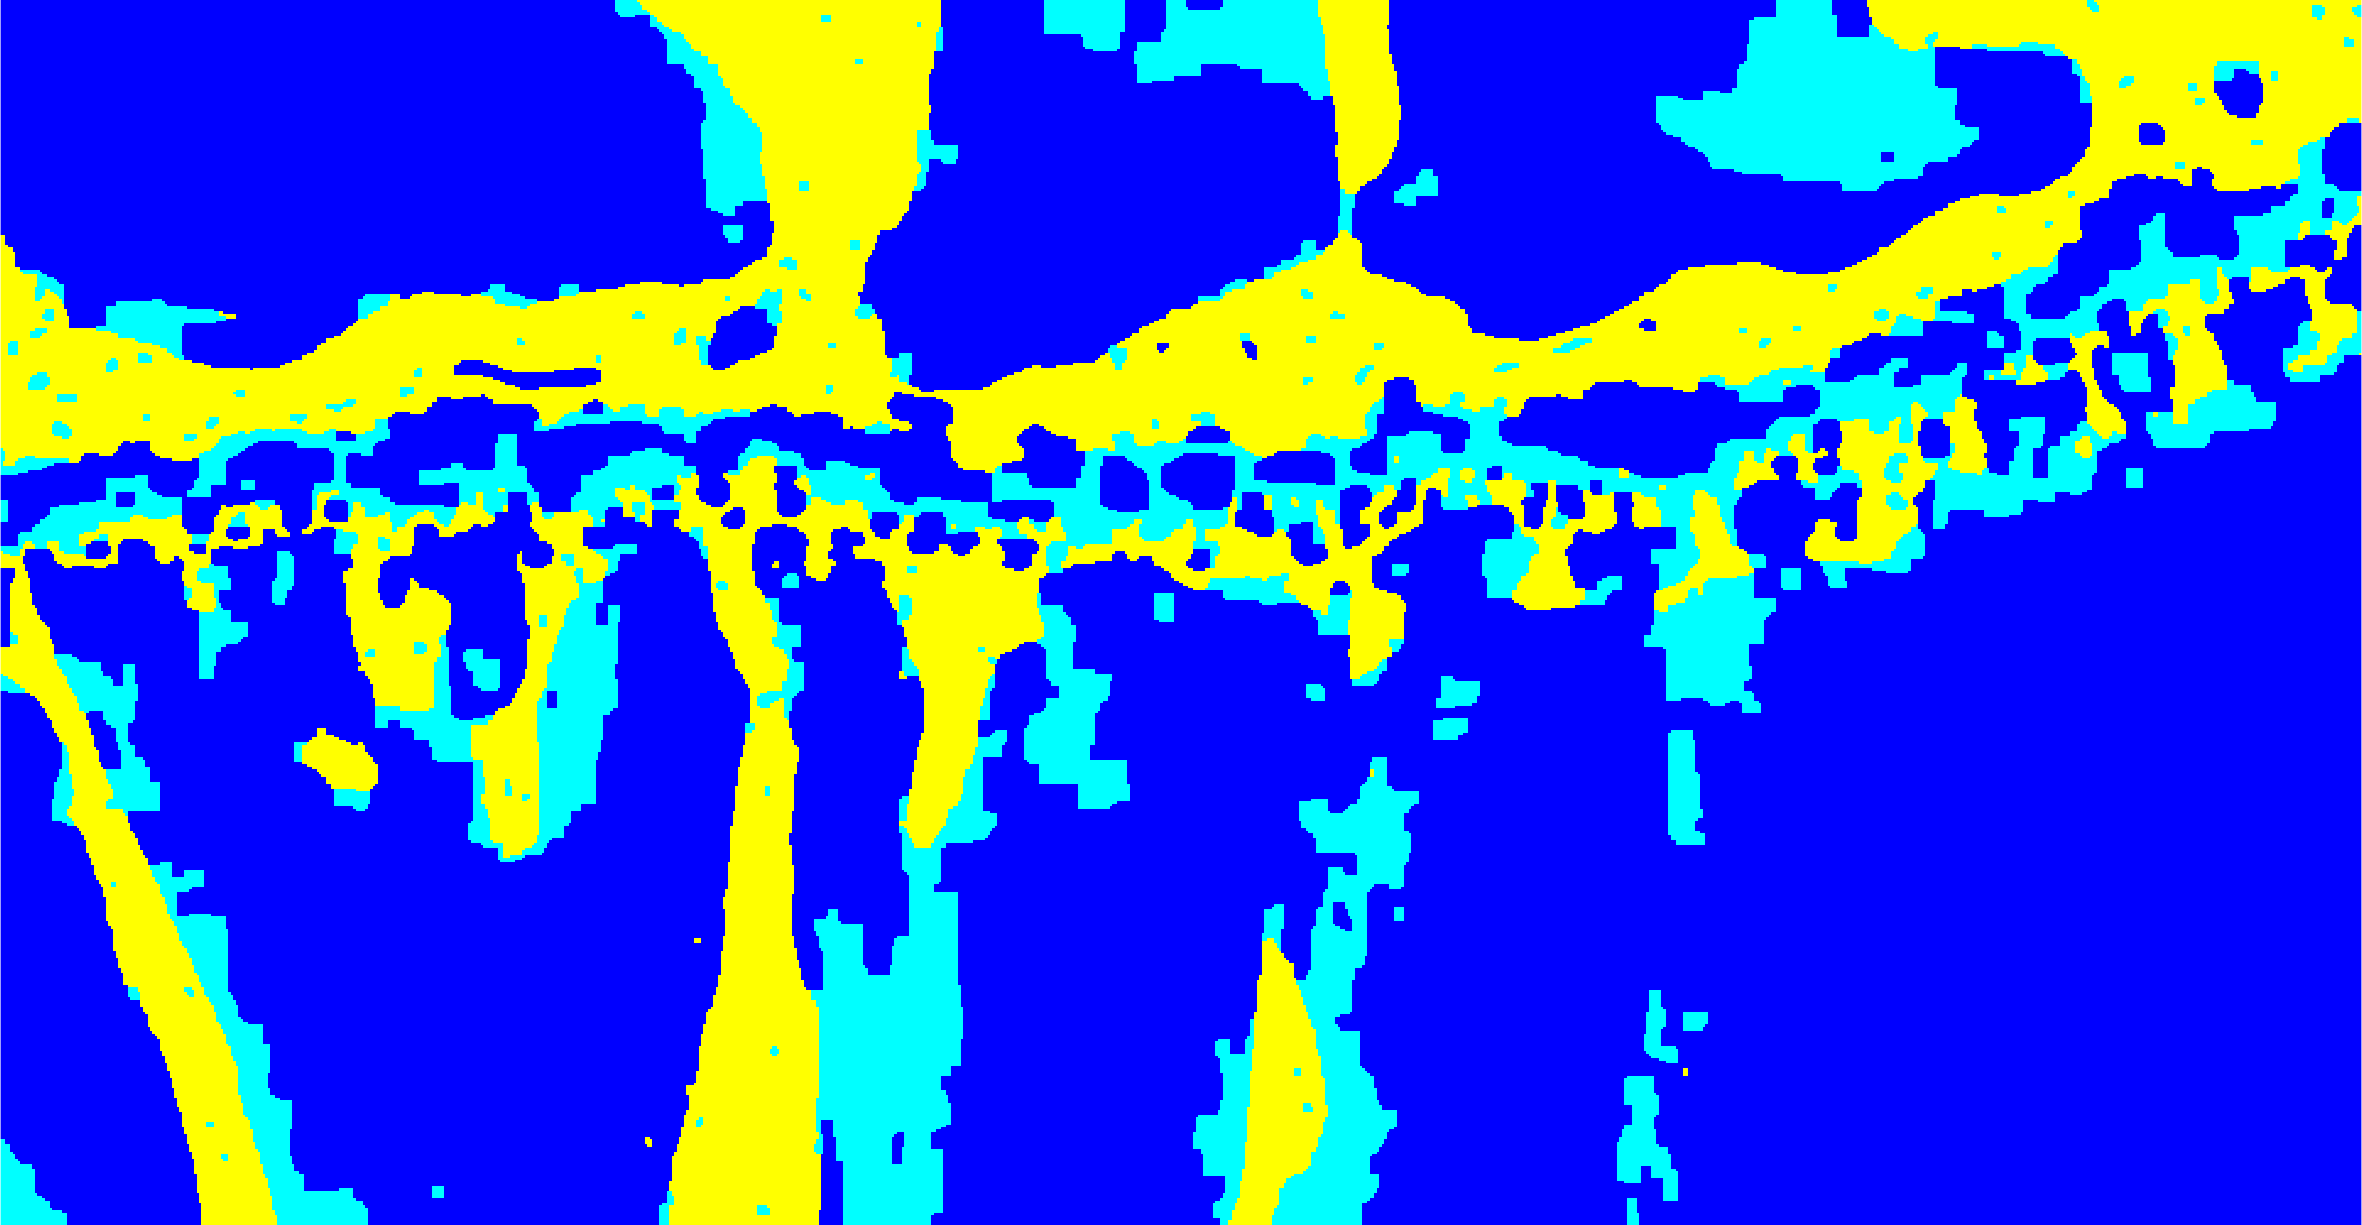
\includegraphics[width=0.5\textwidth]{./figures/assign2_mseg.png}
	\caption{Middle image shows the segmentation of bone (bright) and air (dark). Bottom image shows the segmentation of bone (yellow), cartilage (light blue), and air (dark blue).}
\end{figure}
	\section{Deformable Models}
	\begin{figure}[htbp]
	\centering
	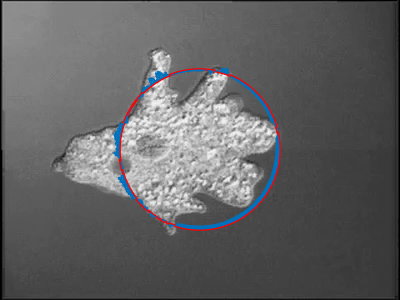
\includegraphics[width=0.45\textwidth]{./figures/defom1.png}
	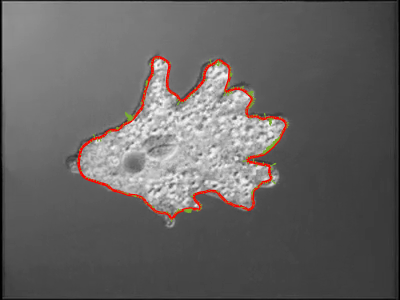
\includegraphics[width=0.45\textwidth]{./figures/defom2.png}
	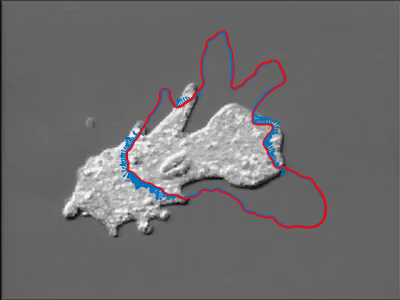
\includegraphics[width=0.45\textwidth]{./figures/defom148.png}
	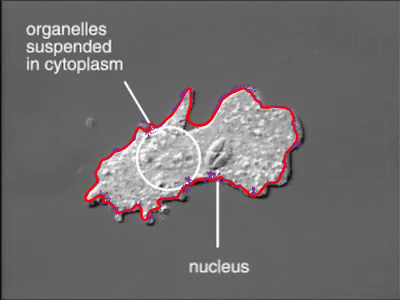
\includegraphics[width=0.45\textwidth]{./figures/defom186.png}
	\caption{Deformable models: top-left is the initial curve, the other three shows the intermediate results.}
\end{figure}
	\section{Geometric Priors}
	Several approaches have been applied for myelinated nerves segmentation, including:
	\begin{enumerate}
	\item Perform MRF segmentation slice by slice. This is done by firstly investigating the histogram of several sample images, and then perform MRF for binary segmentation. Parameters need to be finely tuned in order to have very good results. A snapshot of the final result is shown in Figure~\ref{final1}.
	\begin{figure}[!b]
	\centering
	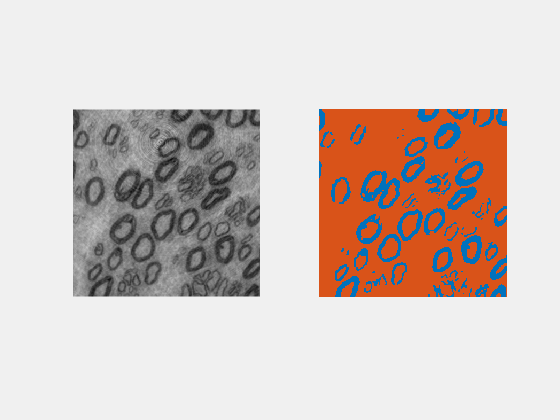
\includegraphics[width=0.8\textwidth]{./figures/1.png}
	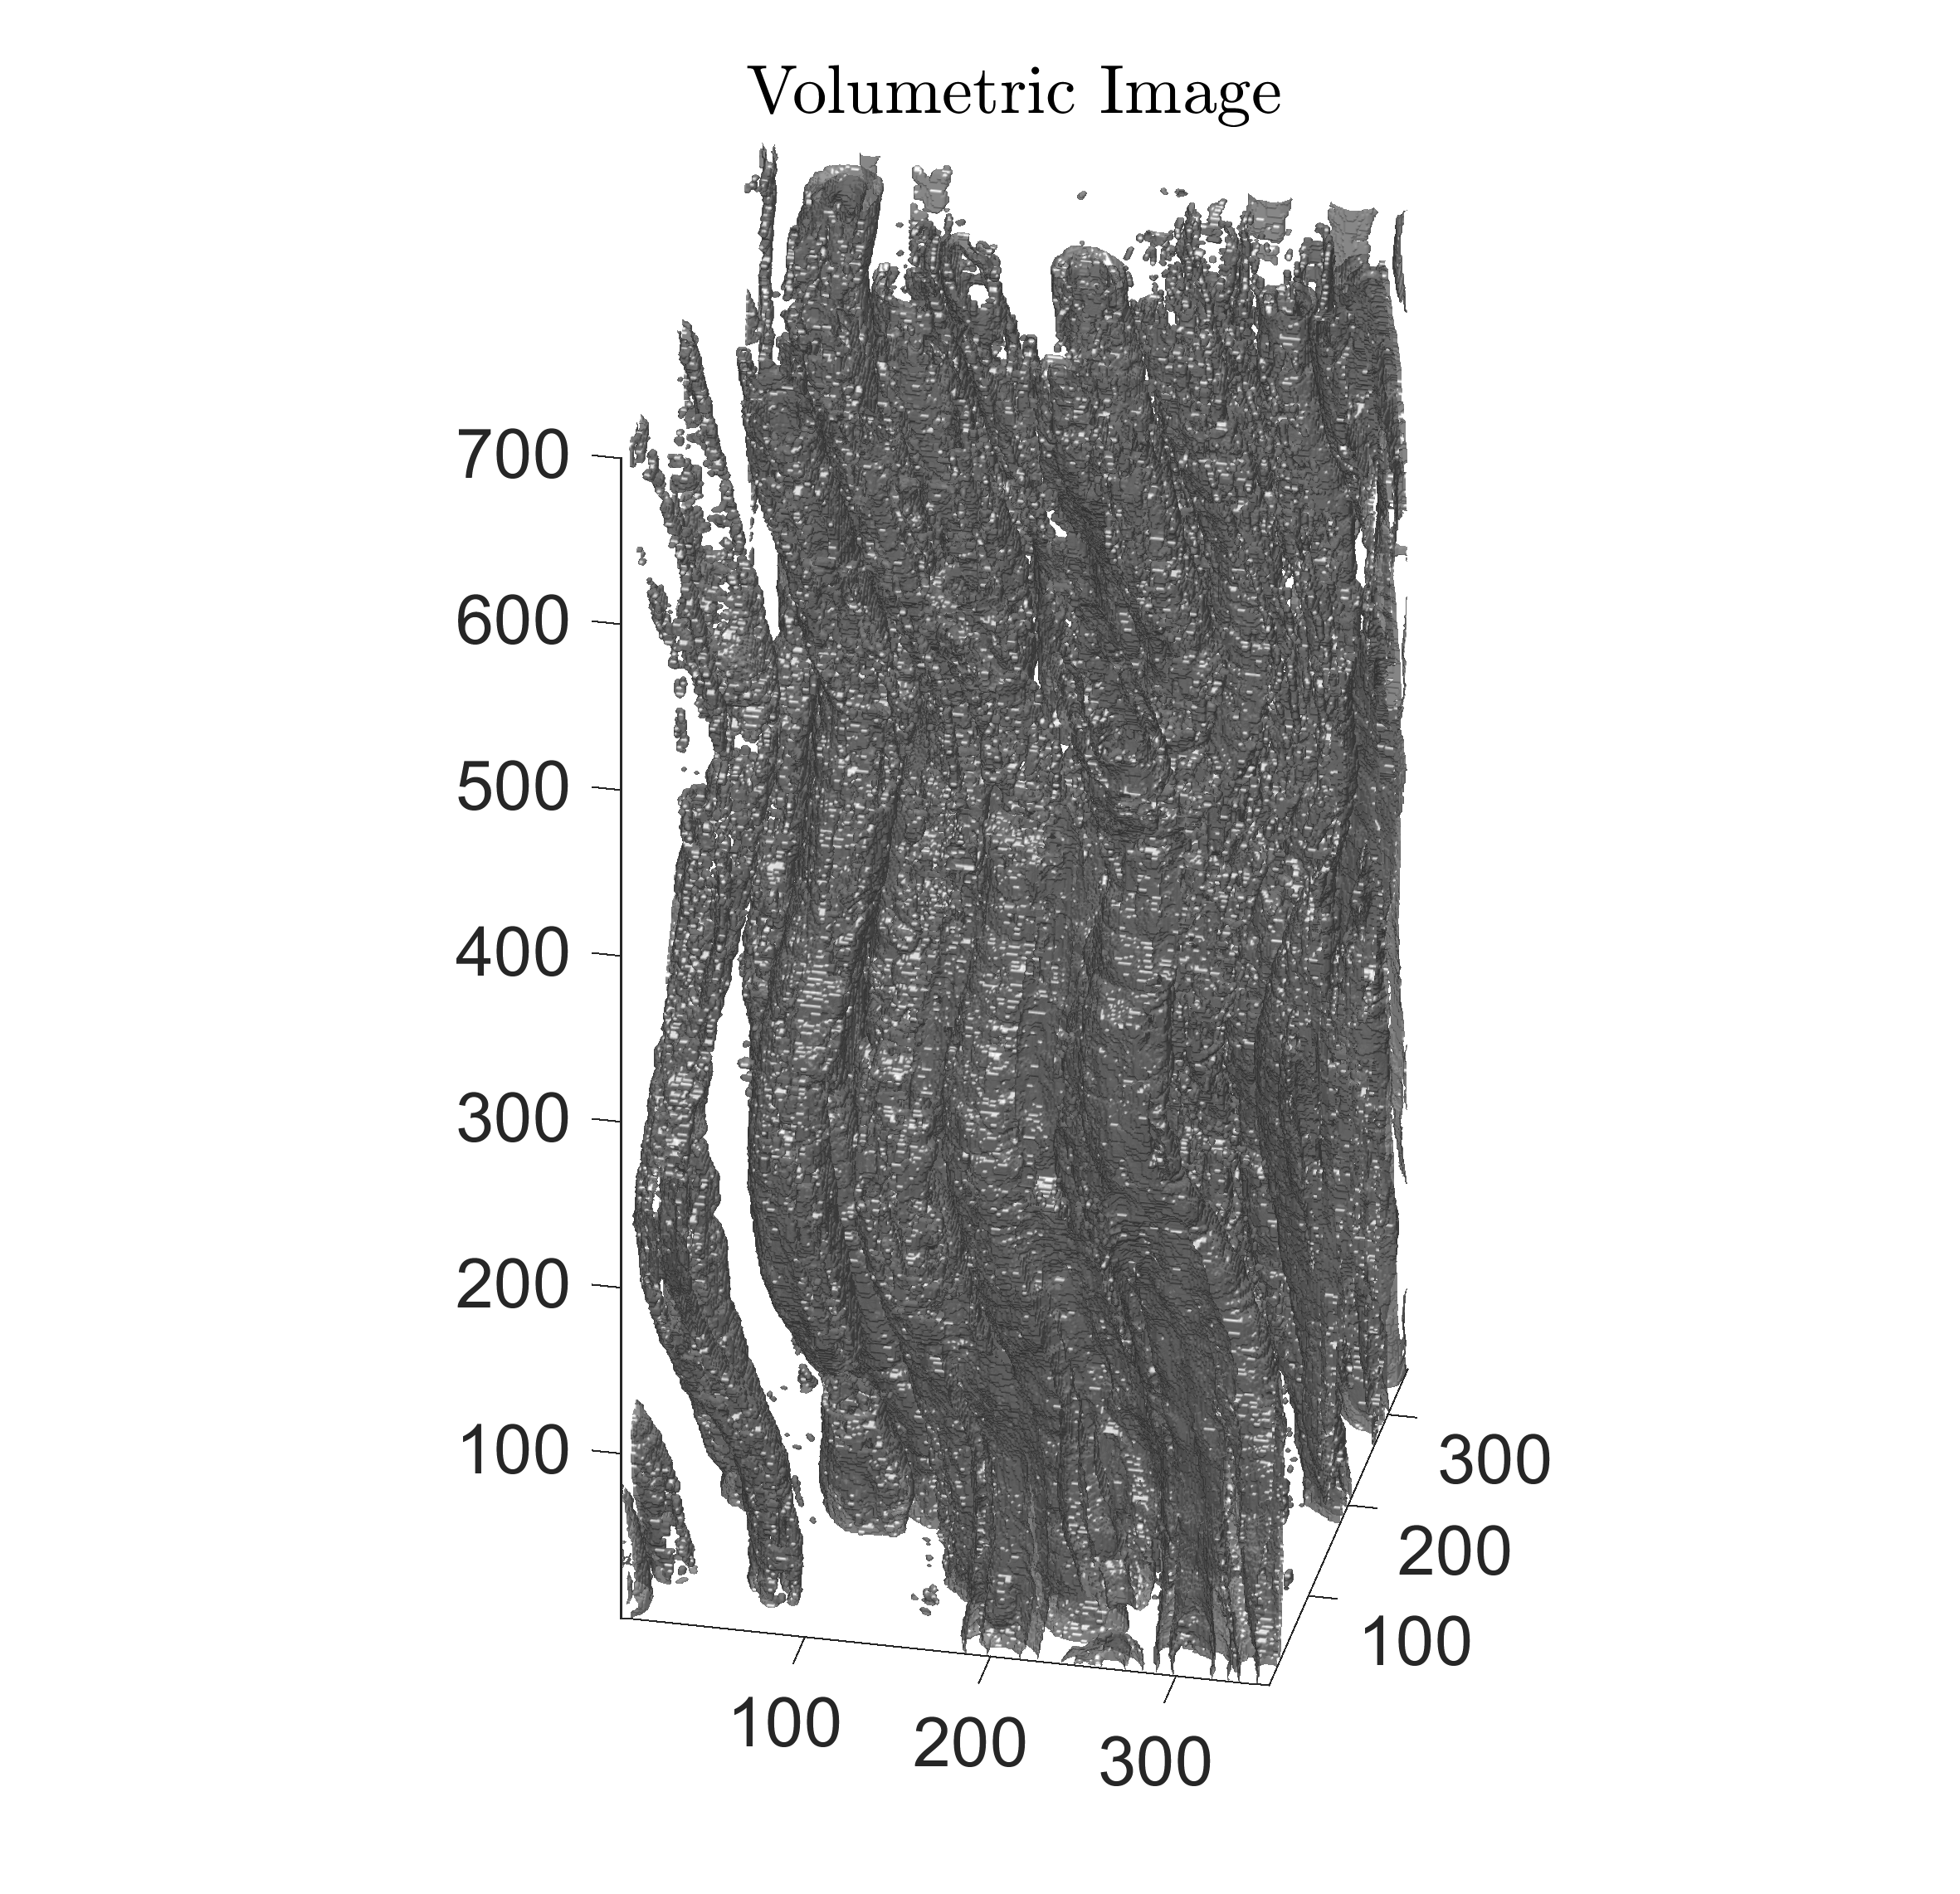
\includegraphics[width=0.8\textwidth]{./figures/final_res1.png}
	\caption{Top image is a snapshot of the slice-by-slice MRF segmentation of nerves image. Bottom image shows the 3D visualization of the segmented nerves.}
	\label{final1}
\end{figure}
	
	\item Perform MRF by considering smoothness among consecutive frames. Theoretically, it is possible to create a full 3D segmentation by stacking all images together. However, because of the memory constraint as well as for saving time, what I did in this assignment is to do the 3D segmentation using $100$ continuous images, i.e. $1-100$ as a batch, $101-200$ as the second batch. A snapshot of the final result is shown in Figure~\ref{final2}.
	
	\begin{figure}[!b]
	\centering
	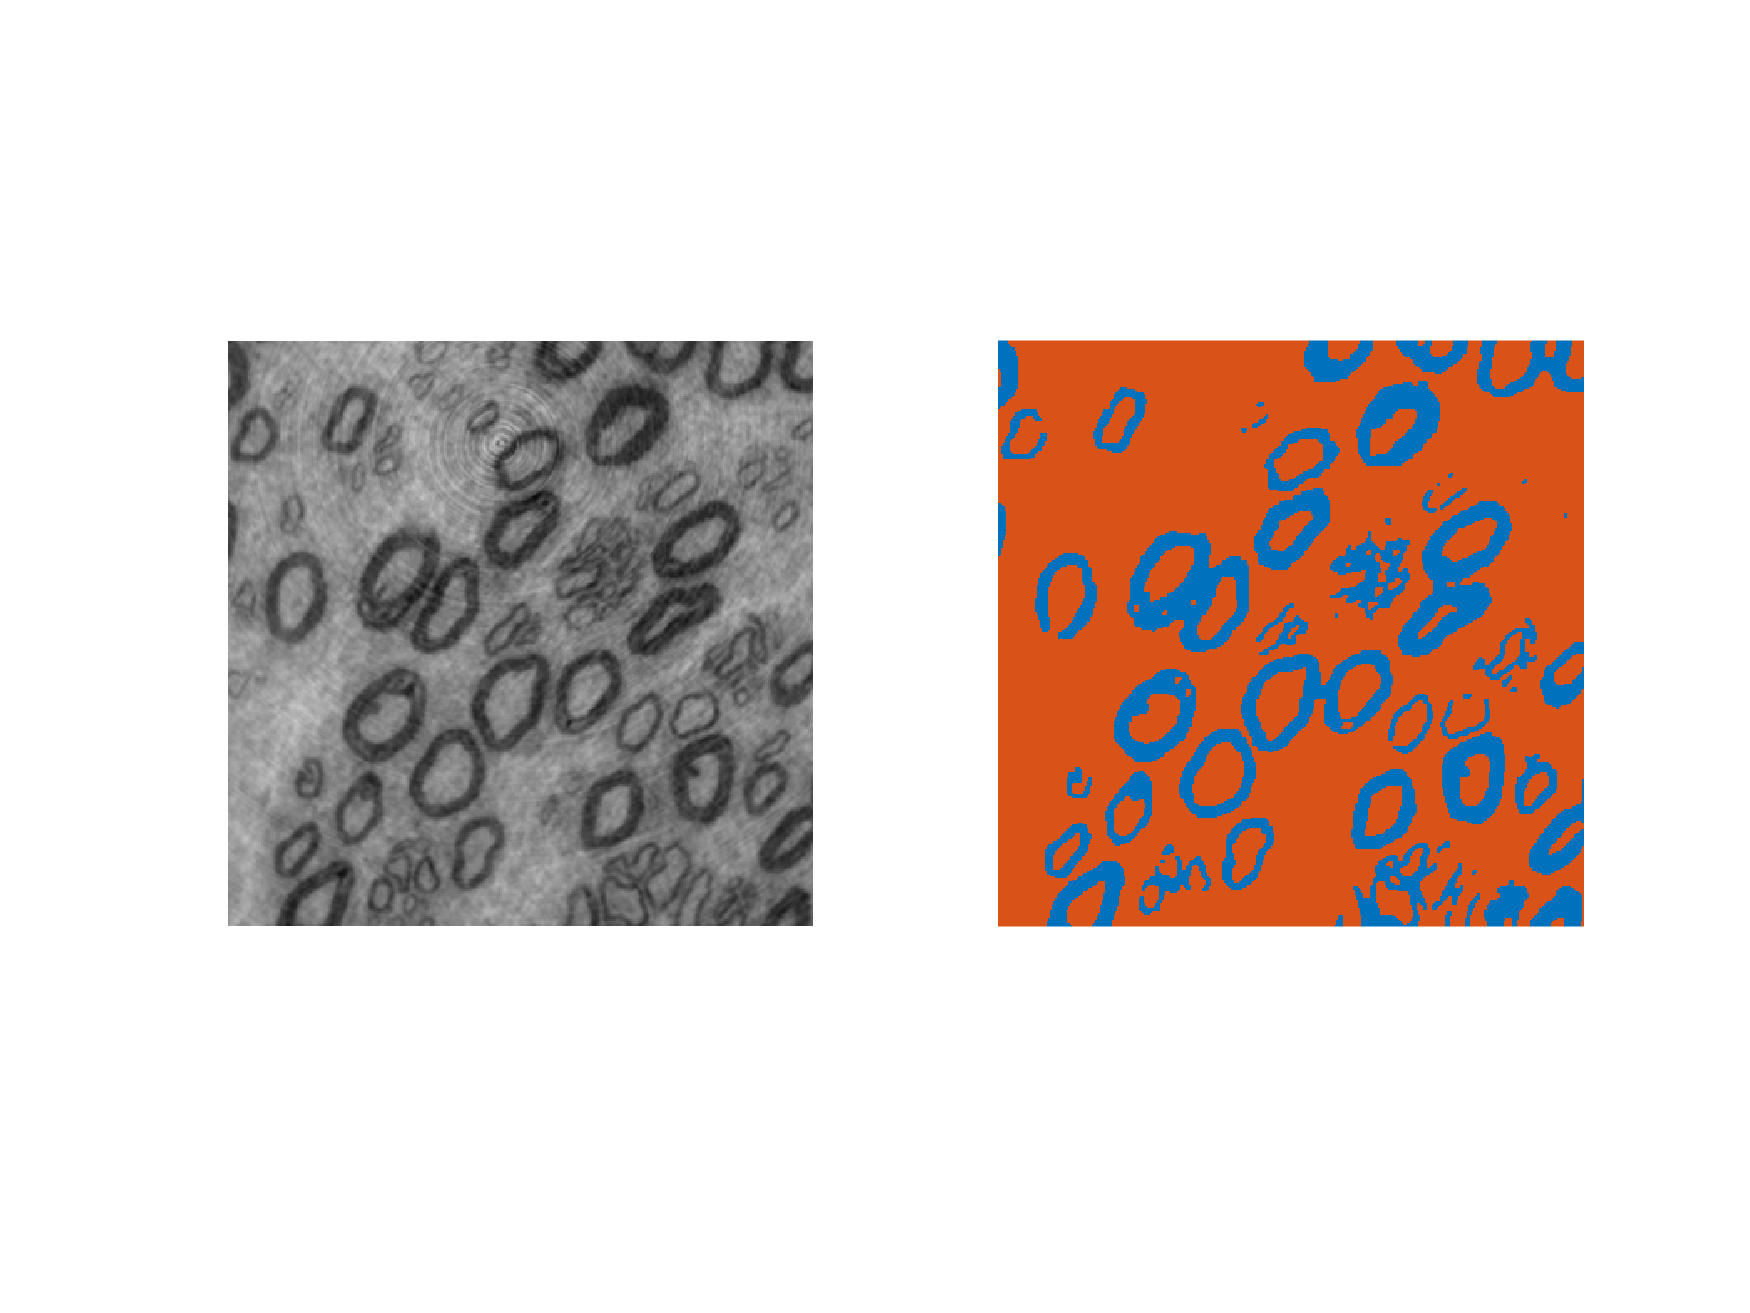
\includegraphics[width=0.8\textwidth]{./figures/2.png}
	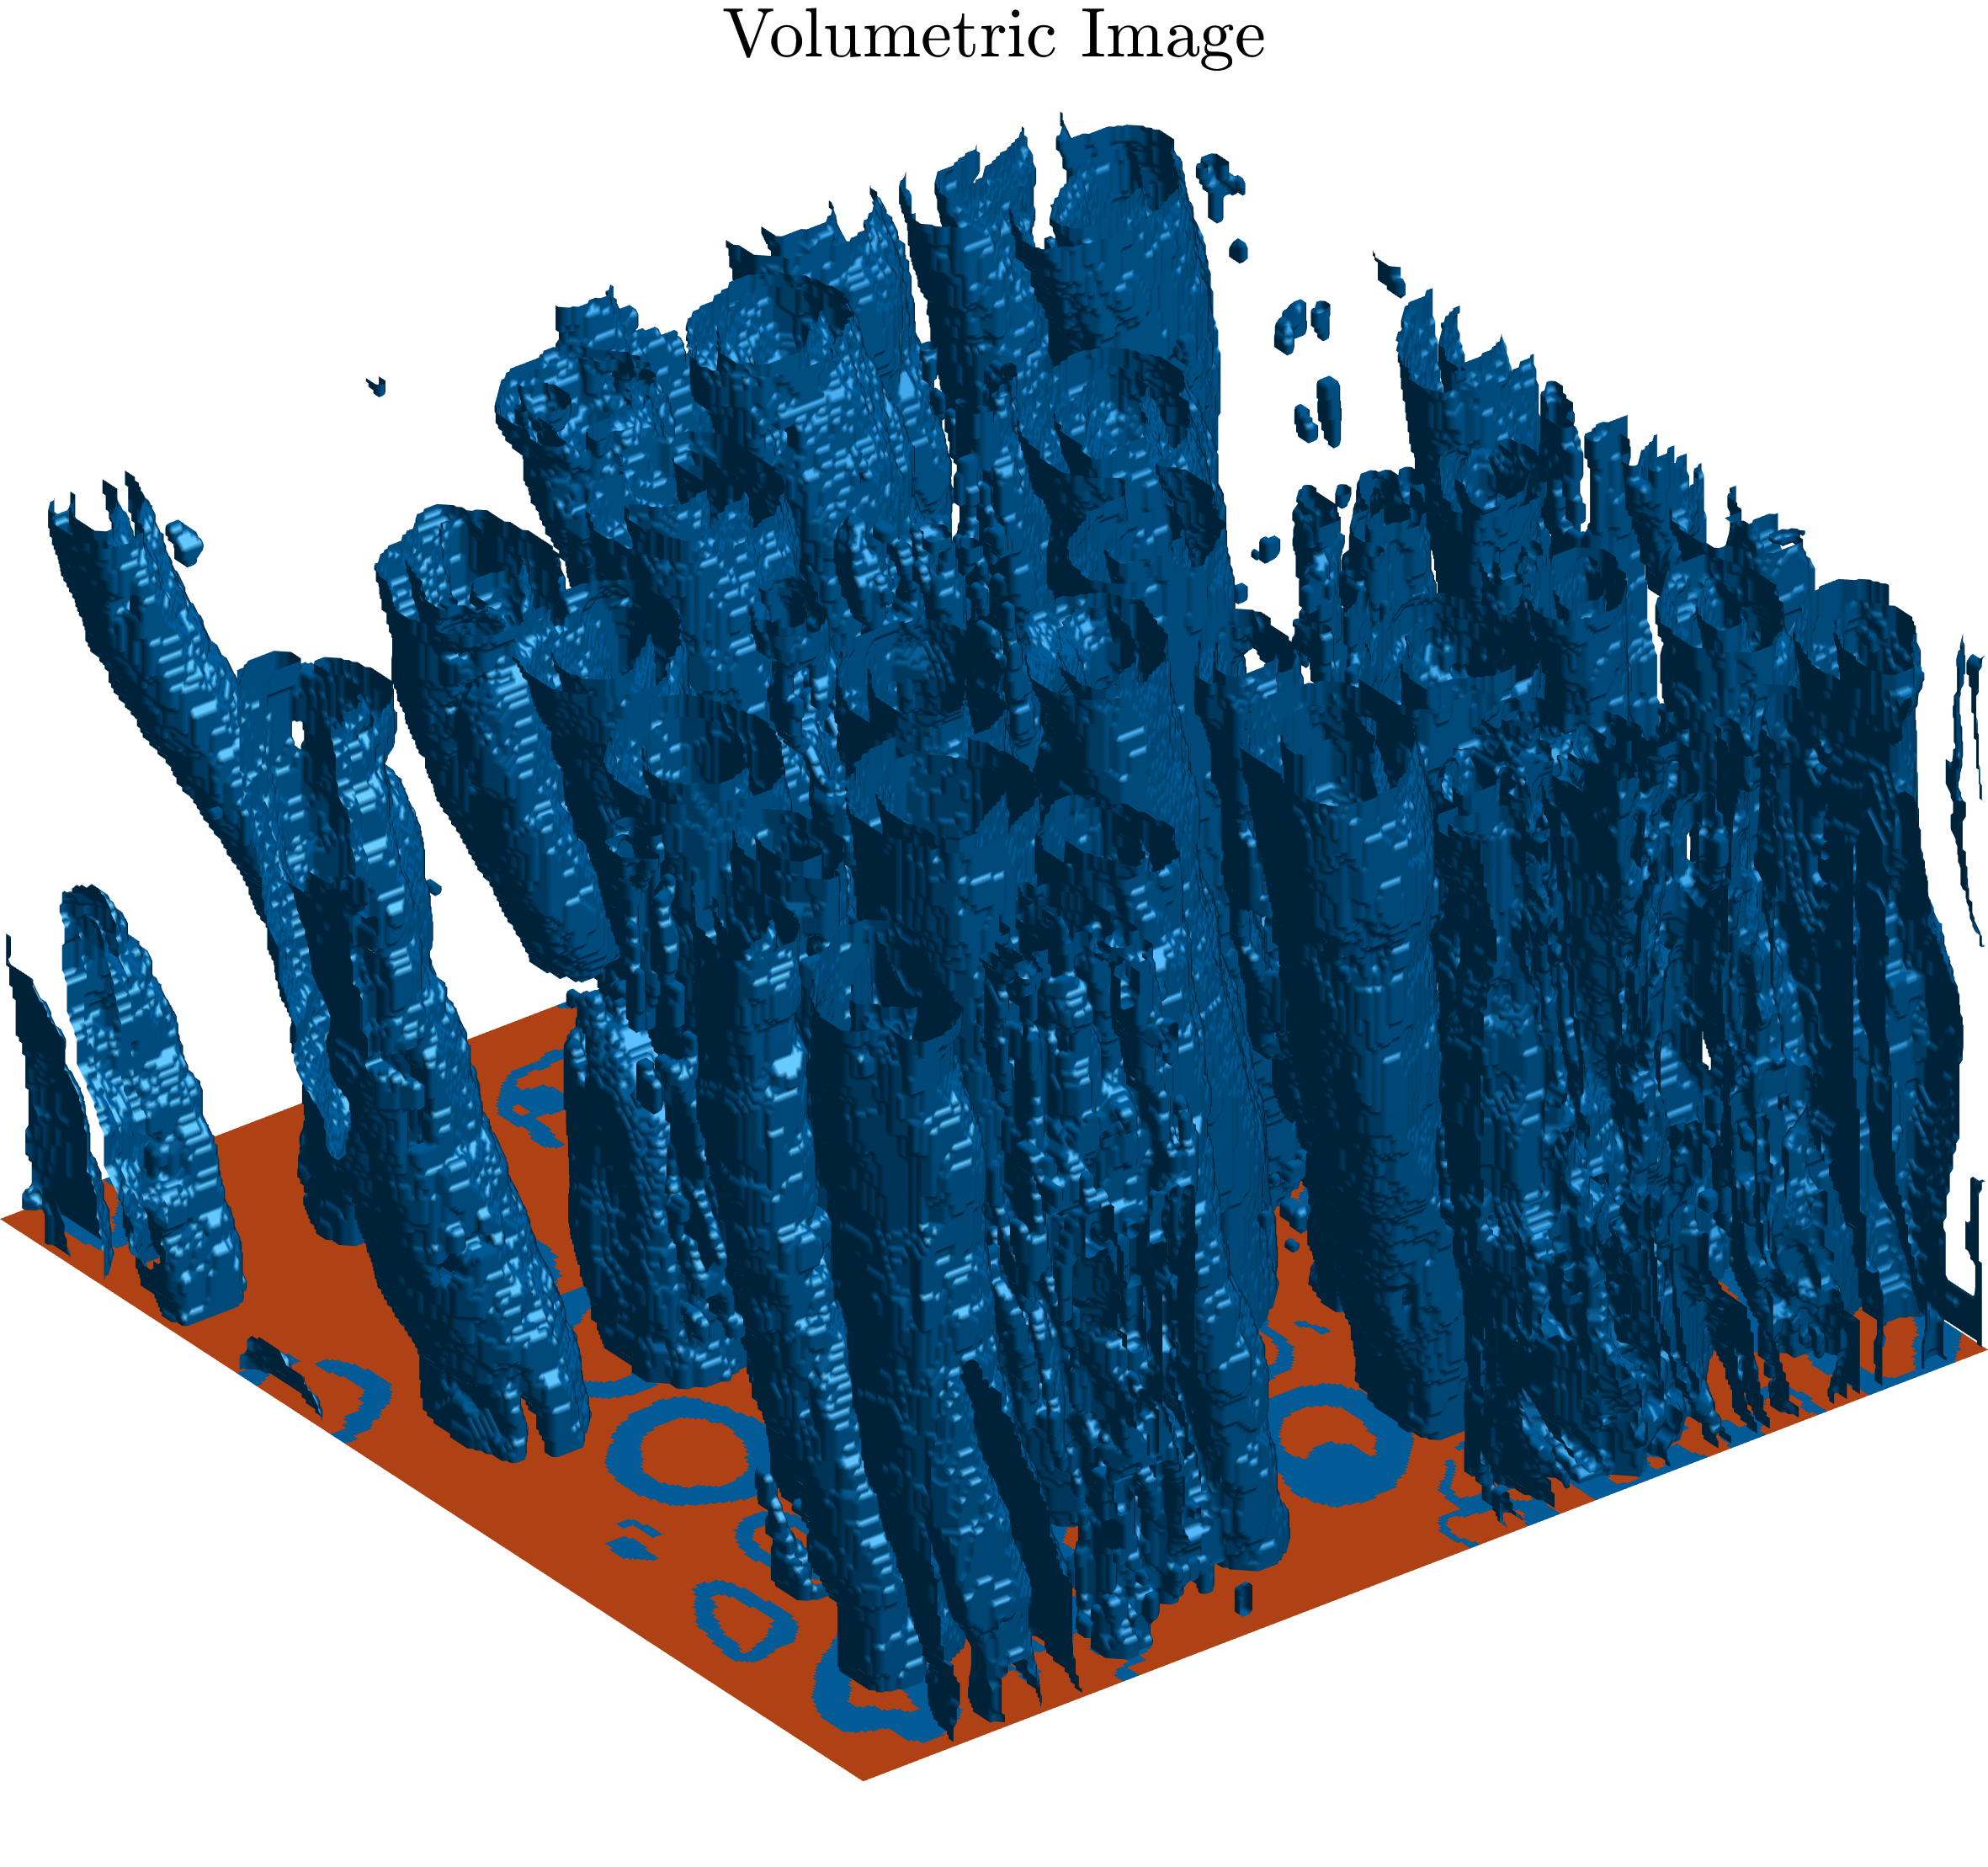
\includegraphics[width=0.8\textwidth]{./figures/final_res2.png}
	\caption{Top image is a snapshot of the $3$D MRF segmentation of nerves image. Bottom image shows the 3D visualization of the segmented nerves (using $1-300$ frames).}
	\label{final2}
\end{figure}	

	\item Perform deformable models using Chan-Vese approach. Since a nerve consists of a dark myelin and a bright axon, $m_{in}$ and $m_{out}$ have to be estimated from a thin band inside and outside the curve. In order to implement this modification without adding too many computational burdens, what I did here are as follows:
	\begin{itemize}
	\item \textit{poly2mask}: find enclosed region of the curve, denoted as $mask_1$;
	\item \textit{findboudary}: self-implemented function for finding boundary of the mask given by a certain curve;
	\item \textit{imdilate}: extend the boundary to its neighbouring pixels by morphological operations, denoted as $mask_2$.
	\item $m_{in}$ and $m_{out}$ can be easily computed by taking the mean intensities of pixels covered by $mask_1\ \&\ mask_2$ and $xor(mask_1\ \&\ mask_2, mask_2)$.
	\item 
	\end{itemize}
	A snapshot of the final result is shown in Figure~\ref{final3}.
	\begin{figure}[!b]
	\centering
	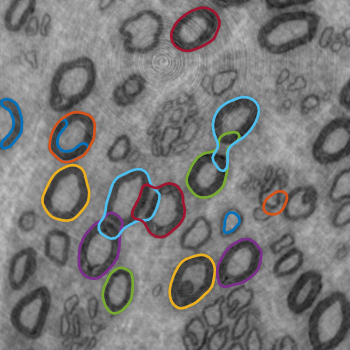
\includegraphics[width=0.5\textwidth]{./figures/257.png}
	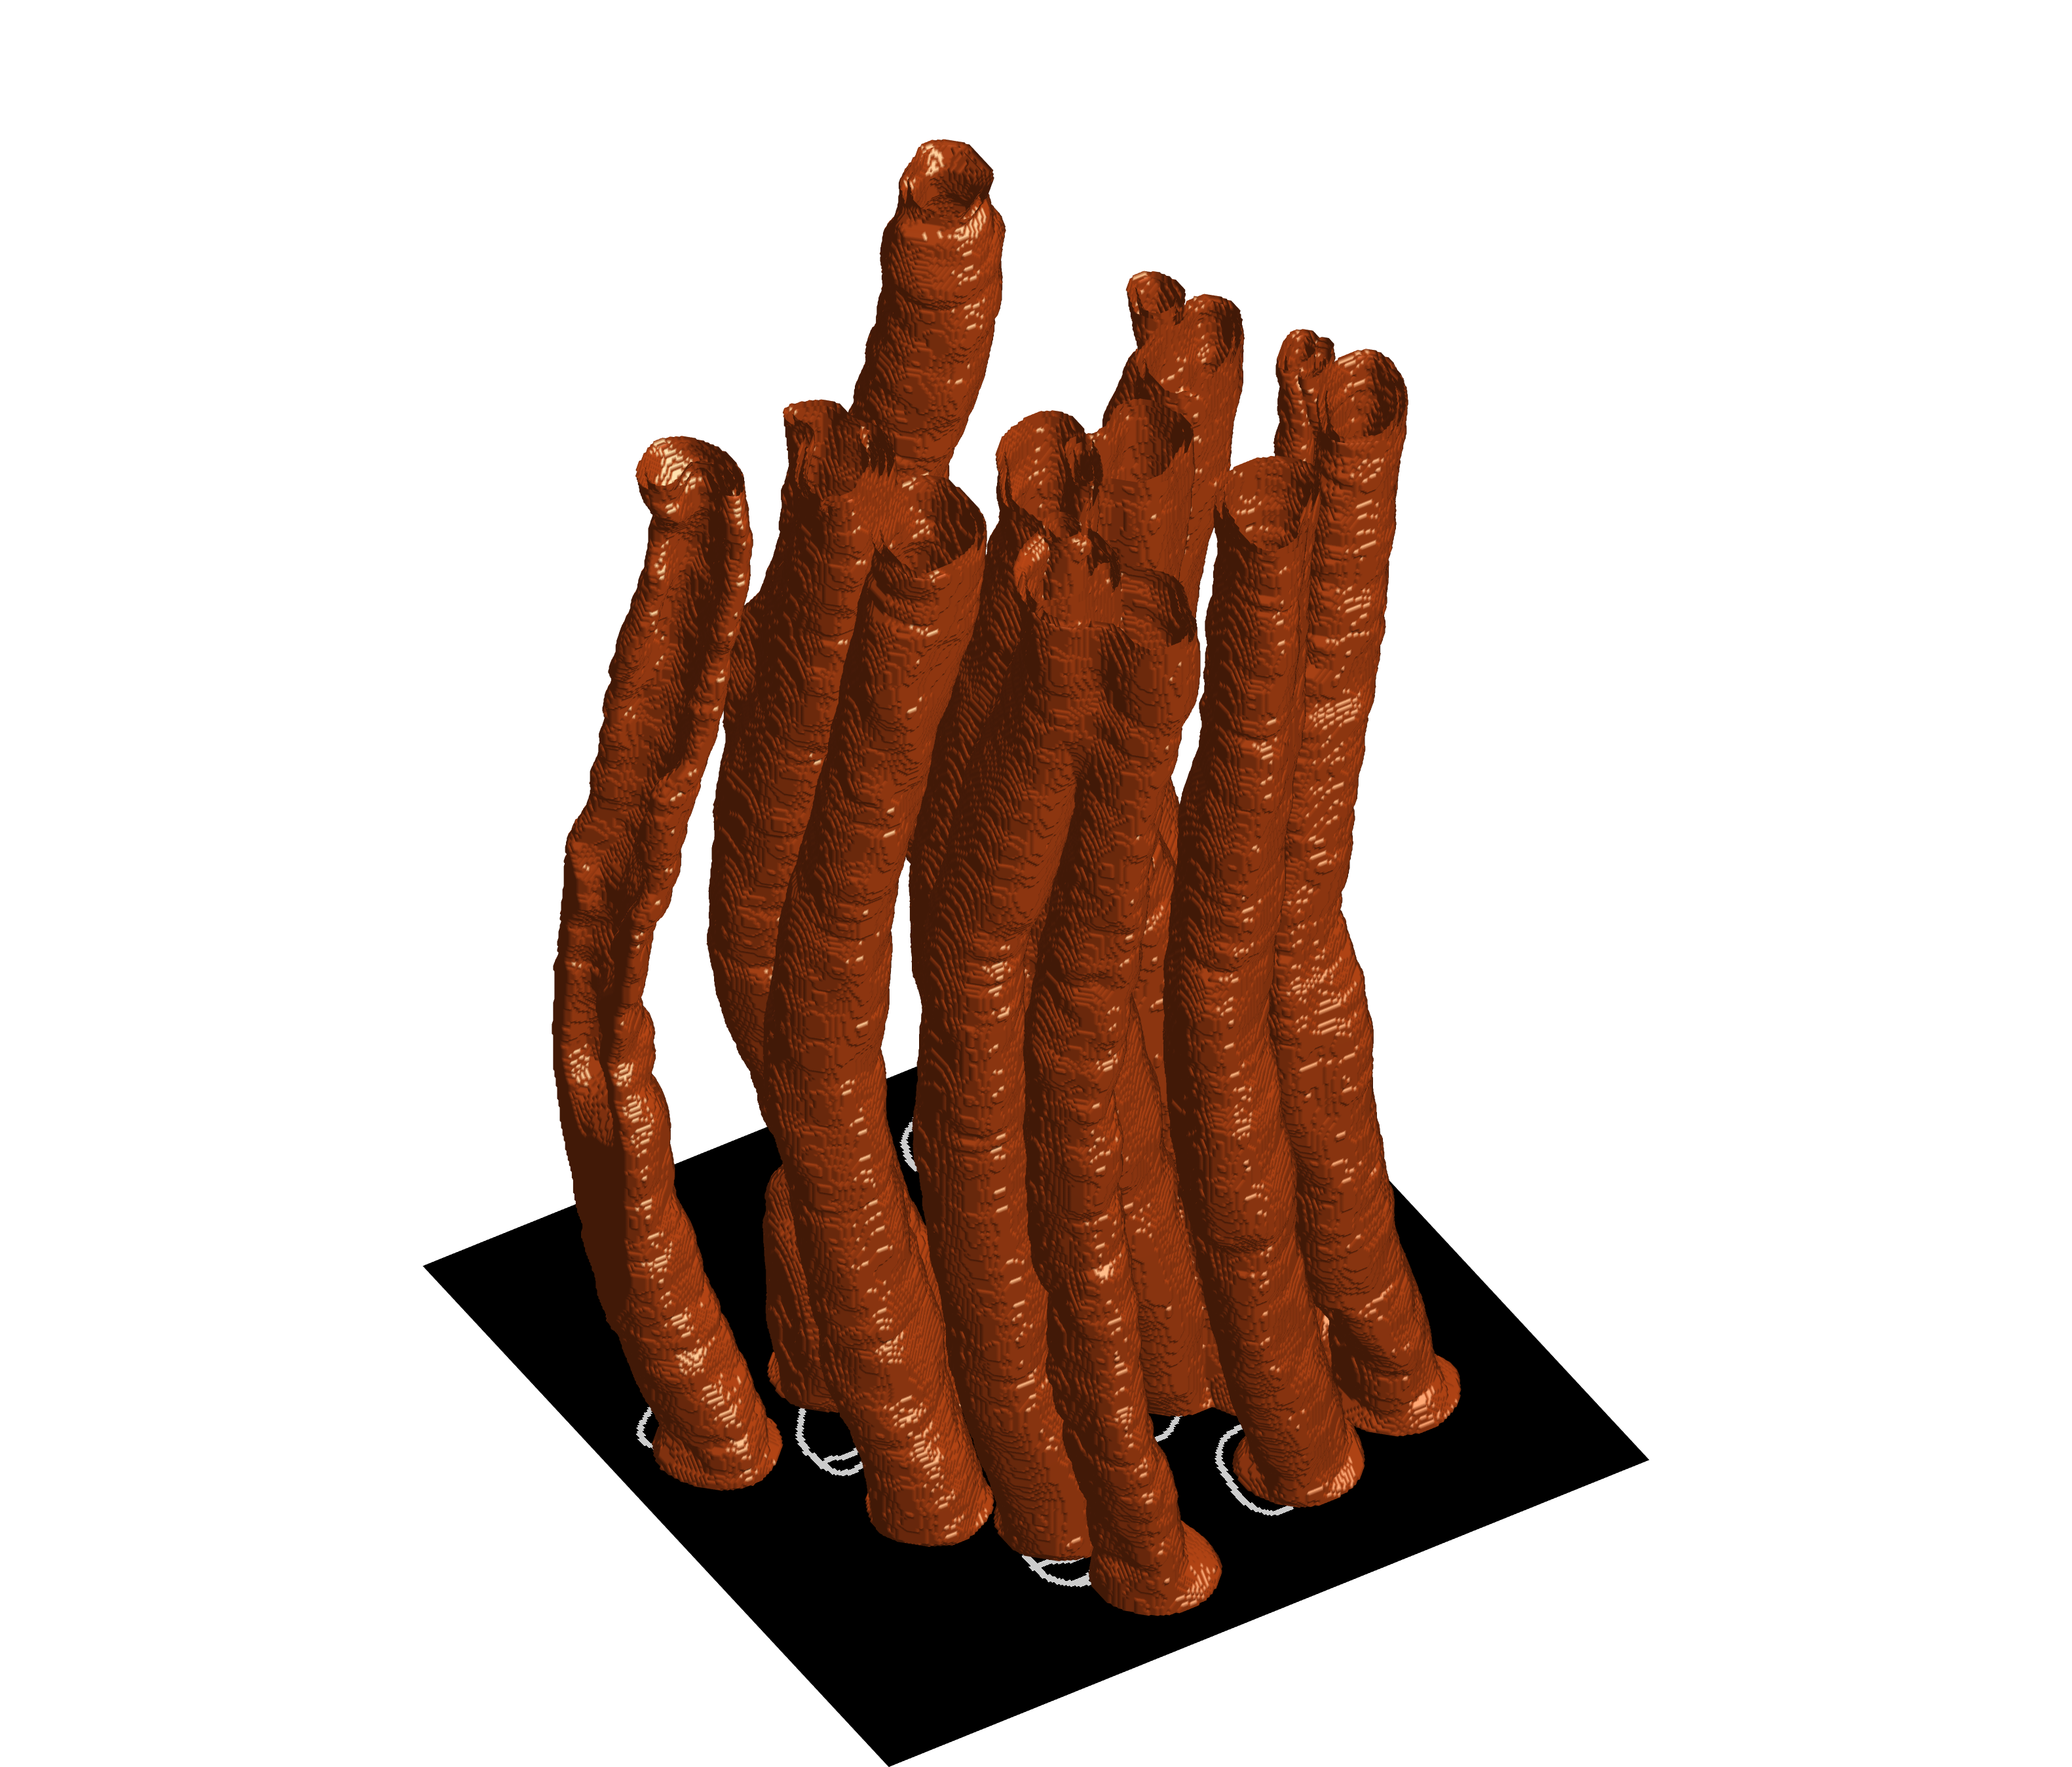
\includegraphics[width=0.8\textwidth]{./figures/final_res3.png}
	\caption{Top image is a snapshot of the segmentation of nerves image using Chan-Vese approach. Bottom image shows the 3D visualization of the segmented nerves (using $1-500$ frames).}
	\label{final3}
\end{figure}		
	
	\end{enumerate}		
	
%https://youtu.be/KMWywGcNNjI	
%https://youtu.be/_GslxUDEZzM

%	Results are shown as follows:
%		\begin{figure}[htbp]
%	\centering
%	\includegraphics[width=0.8\textwidth]{./figures/res1.png}
%	\caption{Blob detection result. Blobs are detected where the local maximas are detected.}
%\end{figure}
%
%\begin{figure}[htbp]
%	\centering
%	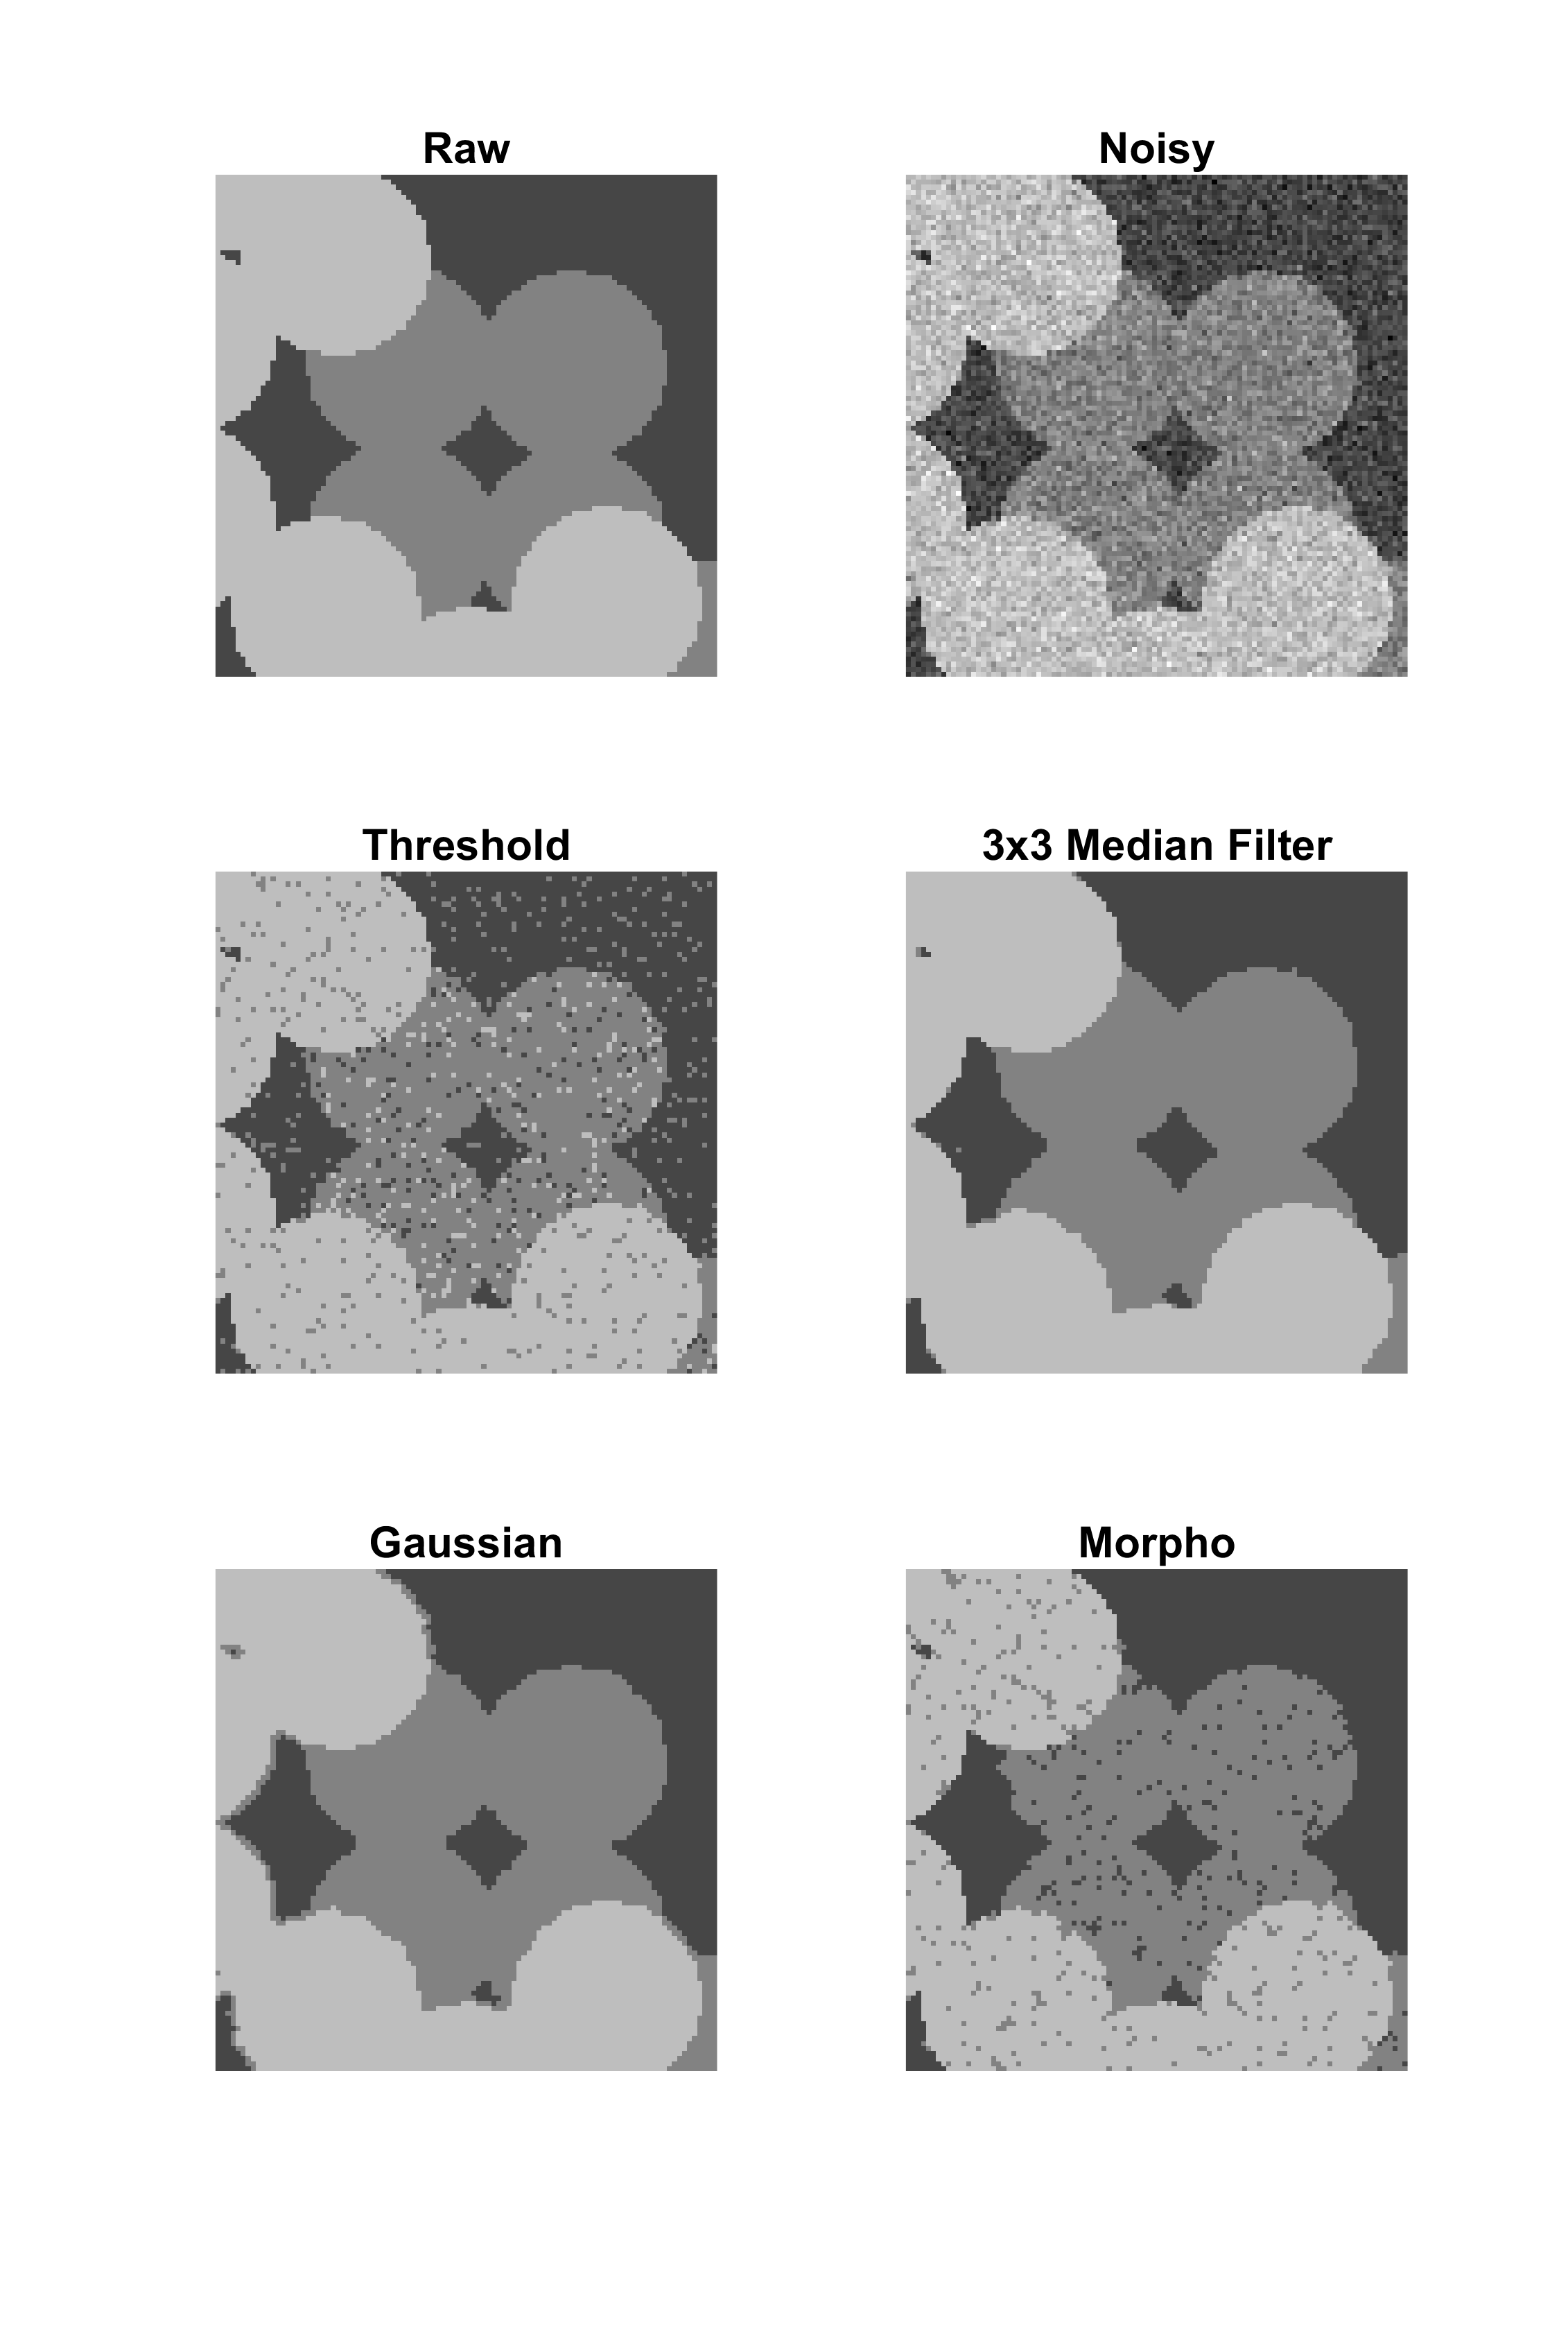
\includegraphics[width=0.8\textwidth]{./figures/res2.png}
%	\caption{Blob detection result. Blobs are detected where the local maximas are detected.}
%\end{figure}
%\begin{figure}[htbp]
%	\centering
%	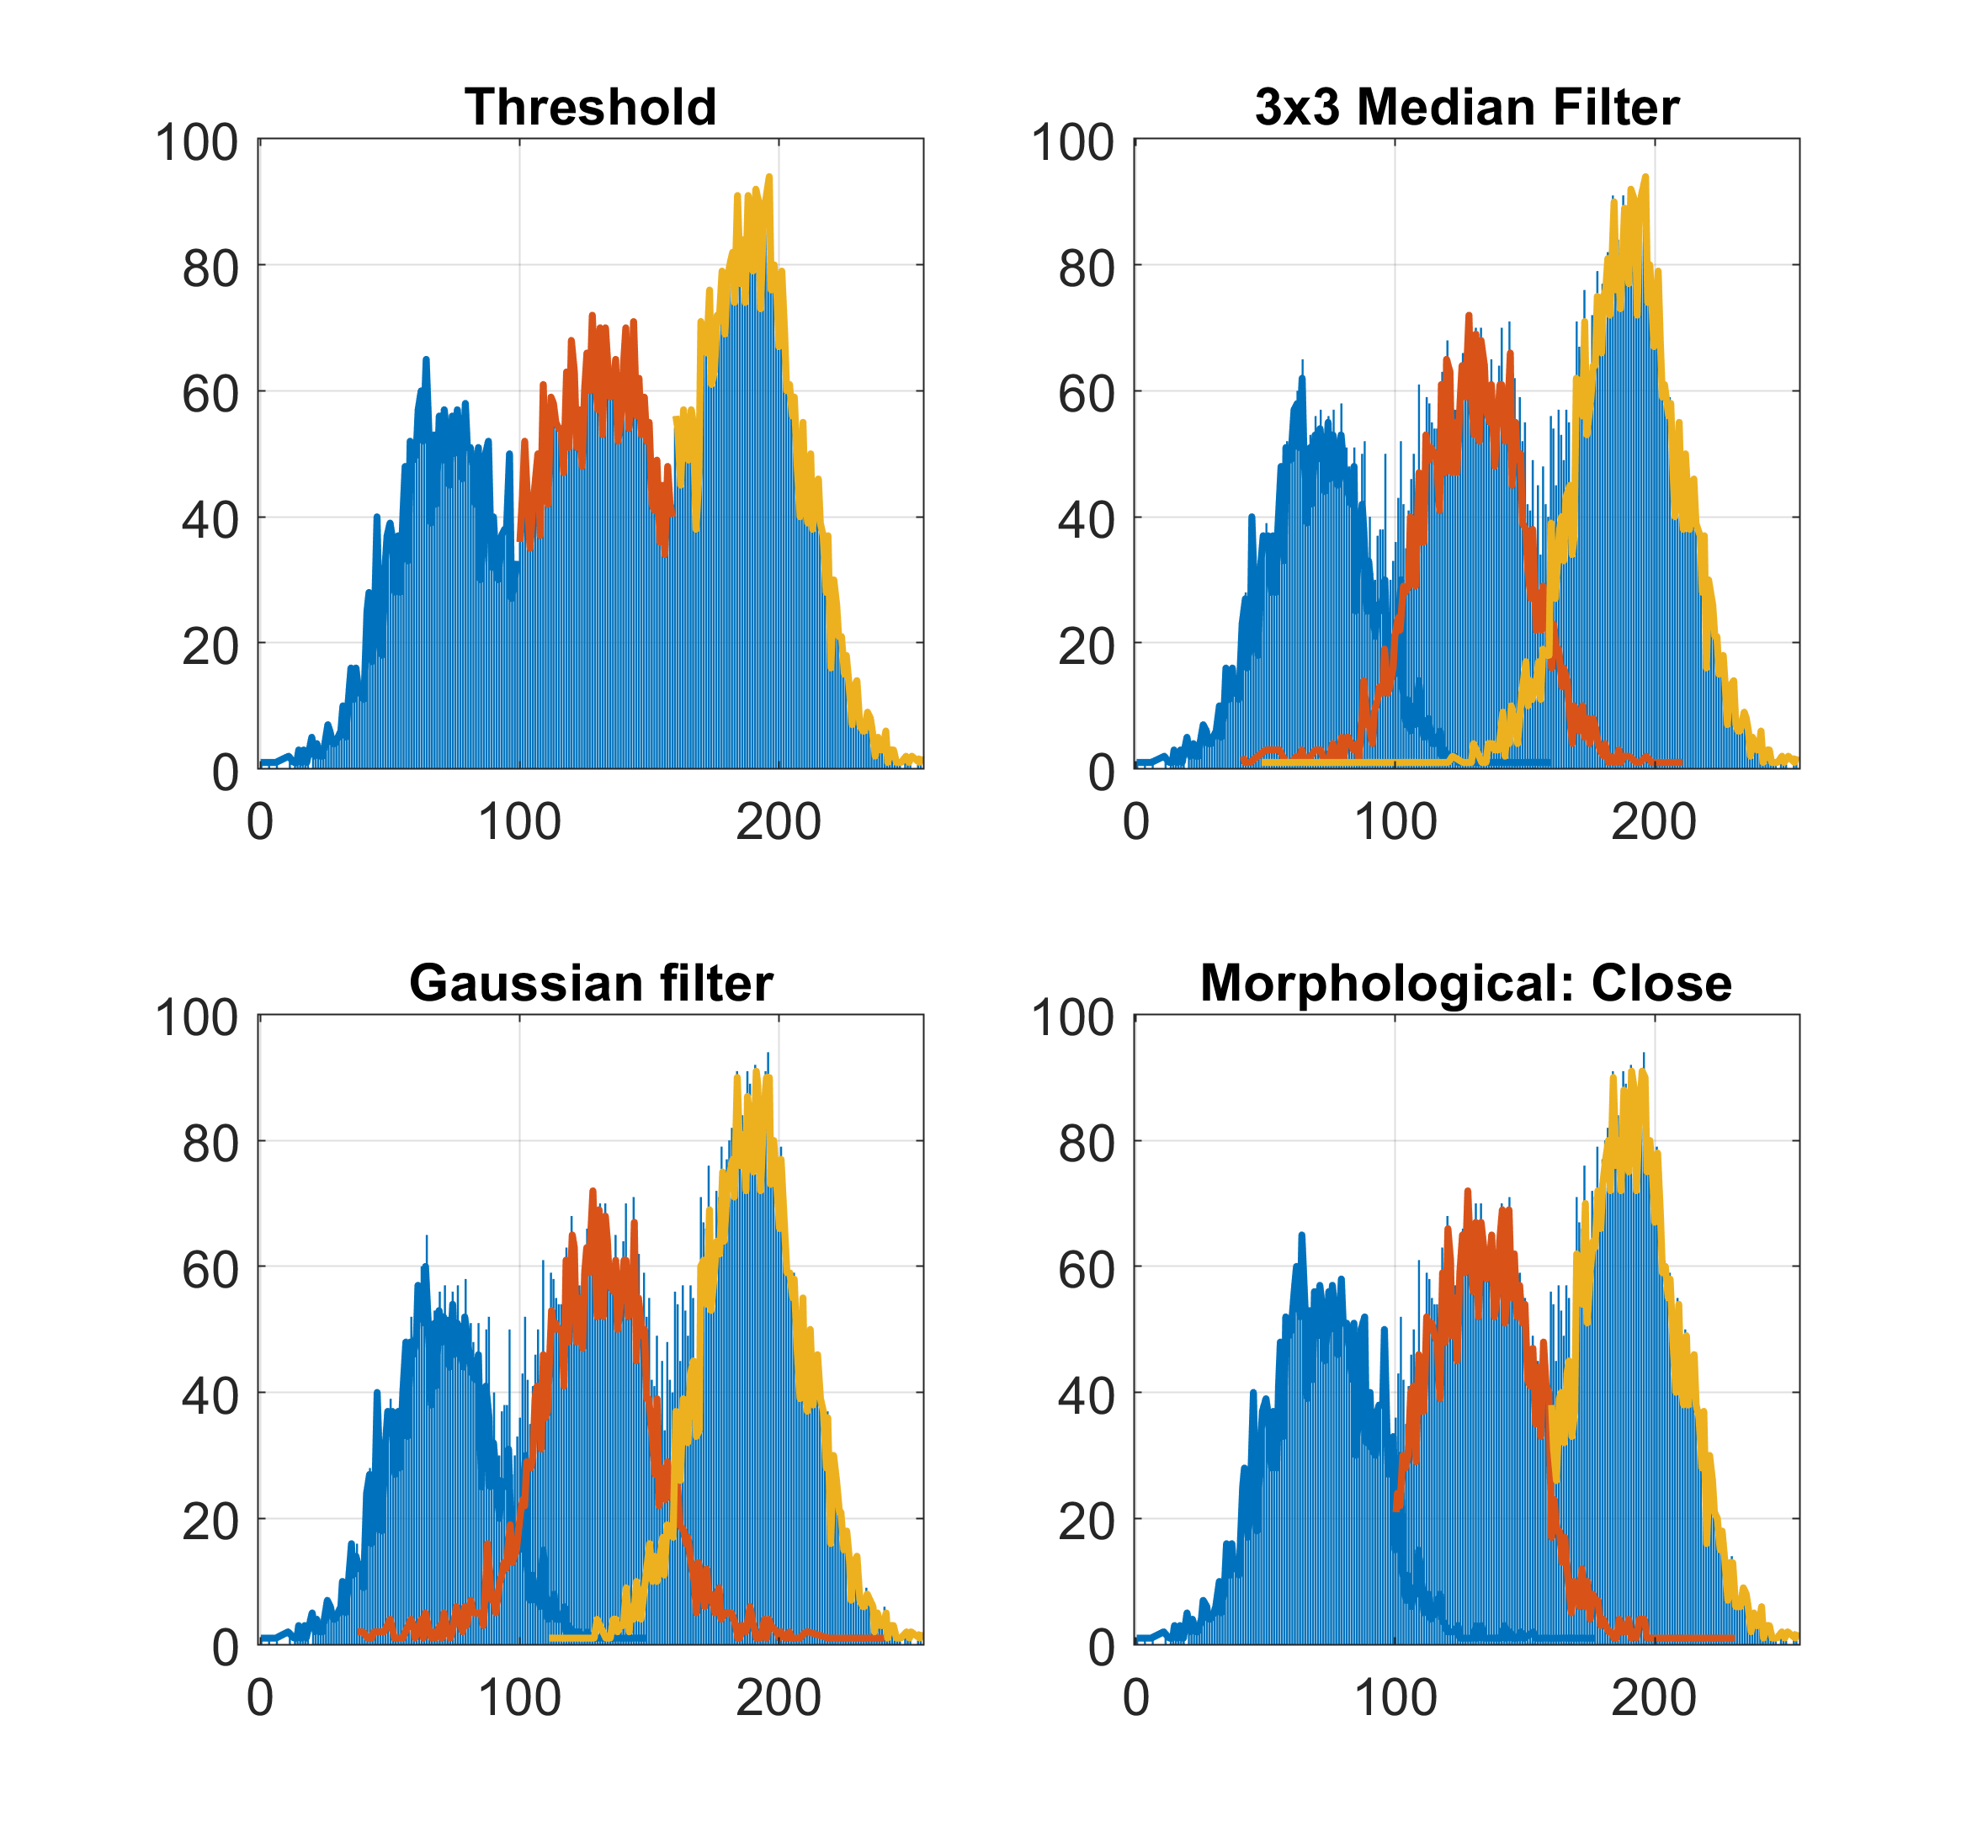
\includegraphics[width=0.8\textwidth]{./figures/res3.png}
%	\caption{Blob detection result. Blobs are detected where the local maximas are detected.}
%\end{figure}
%\begin{figure}[htbp]
%	\centering
%	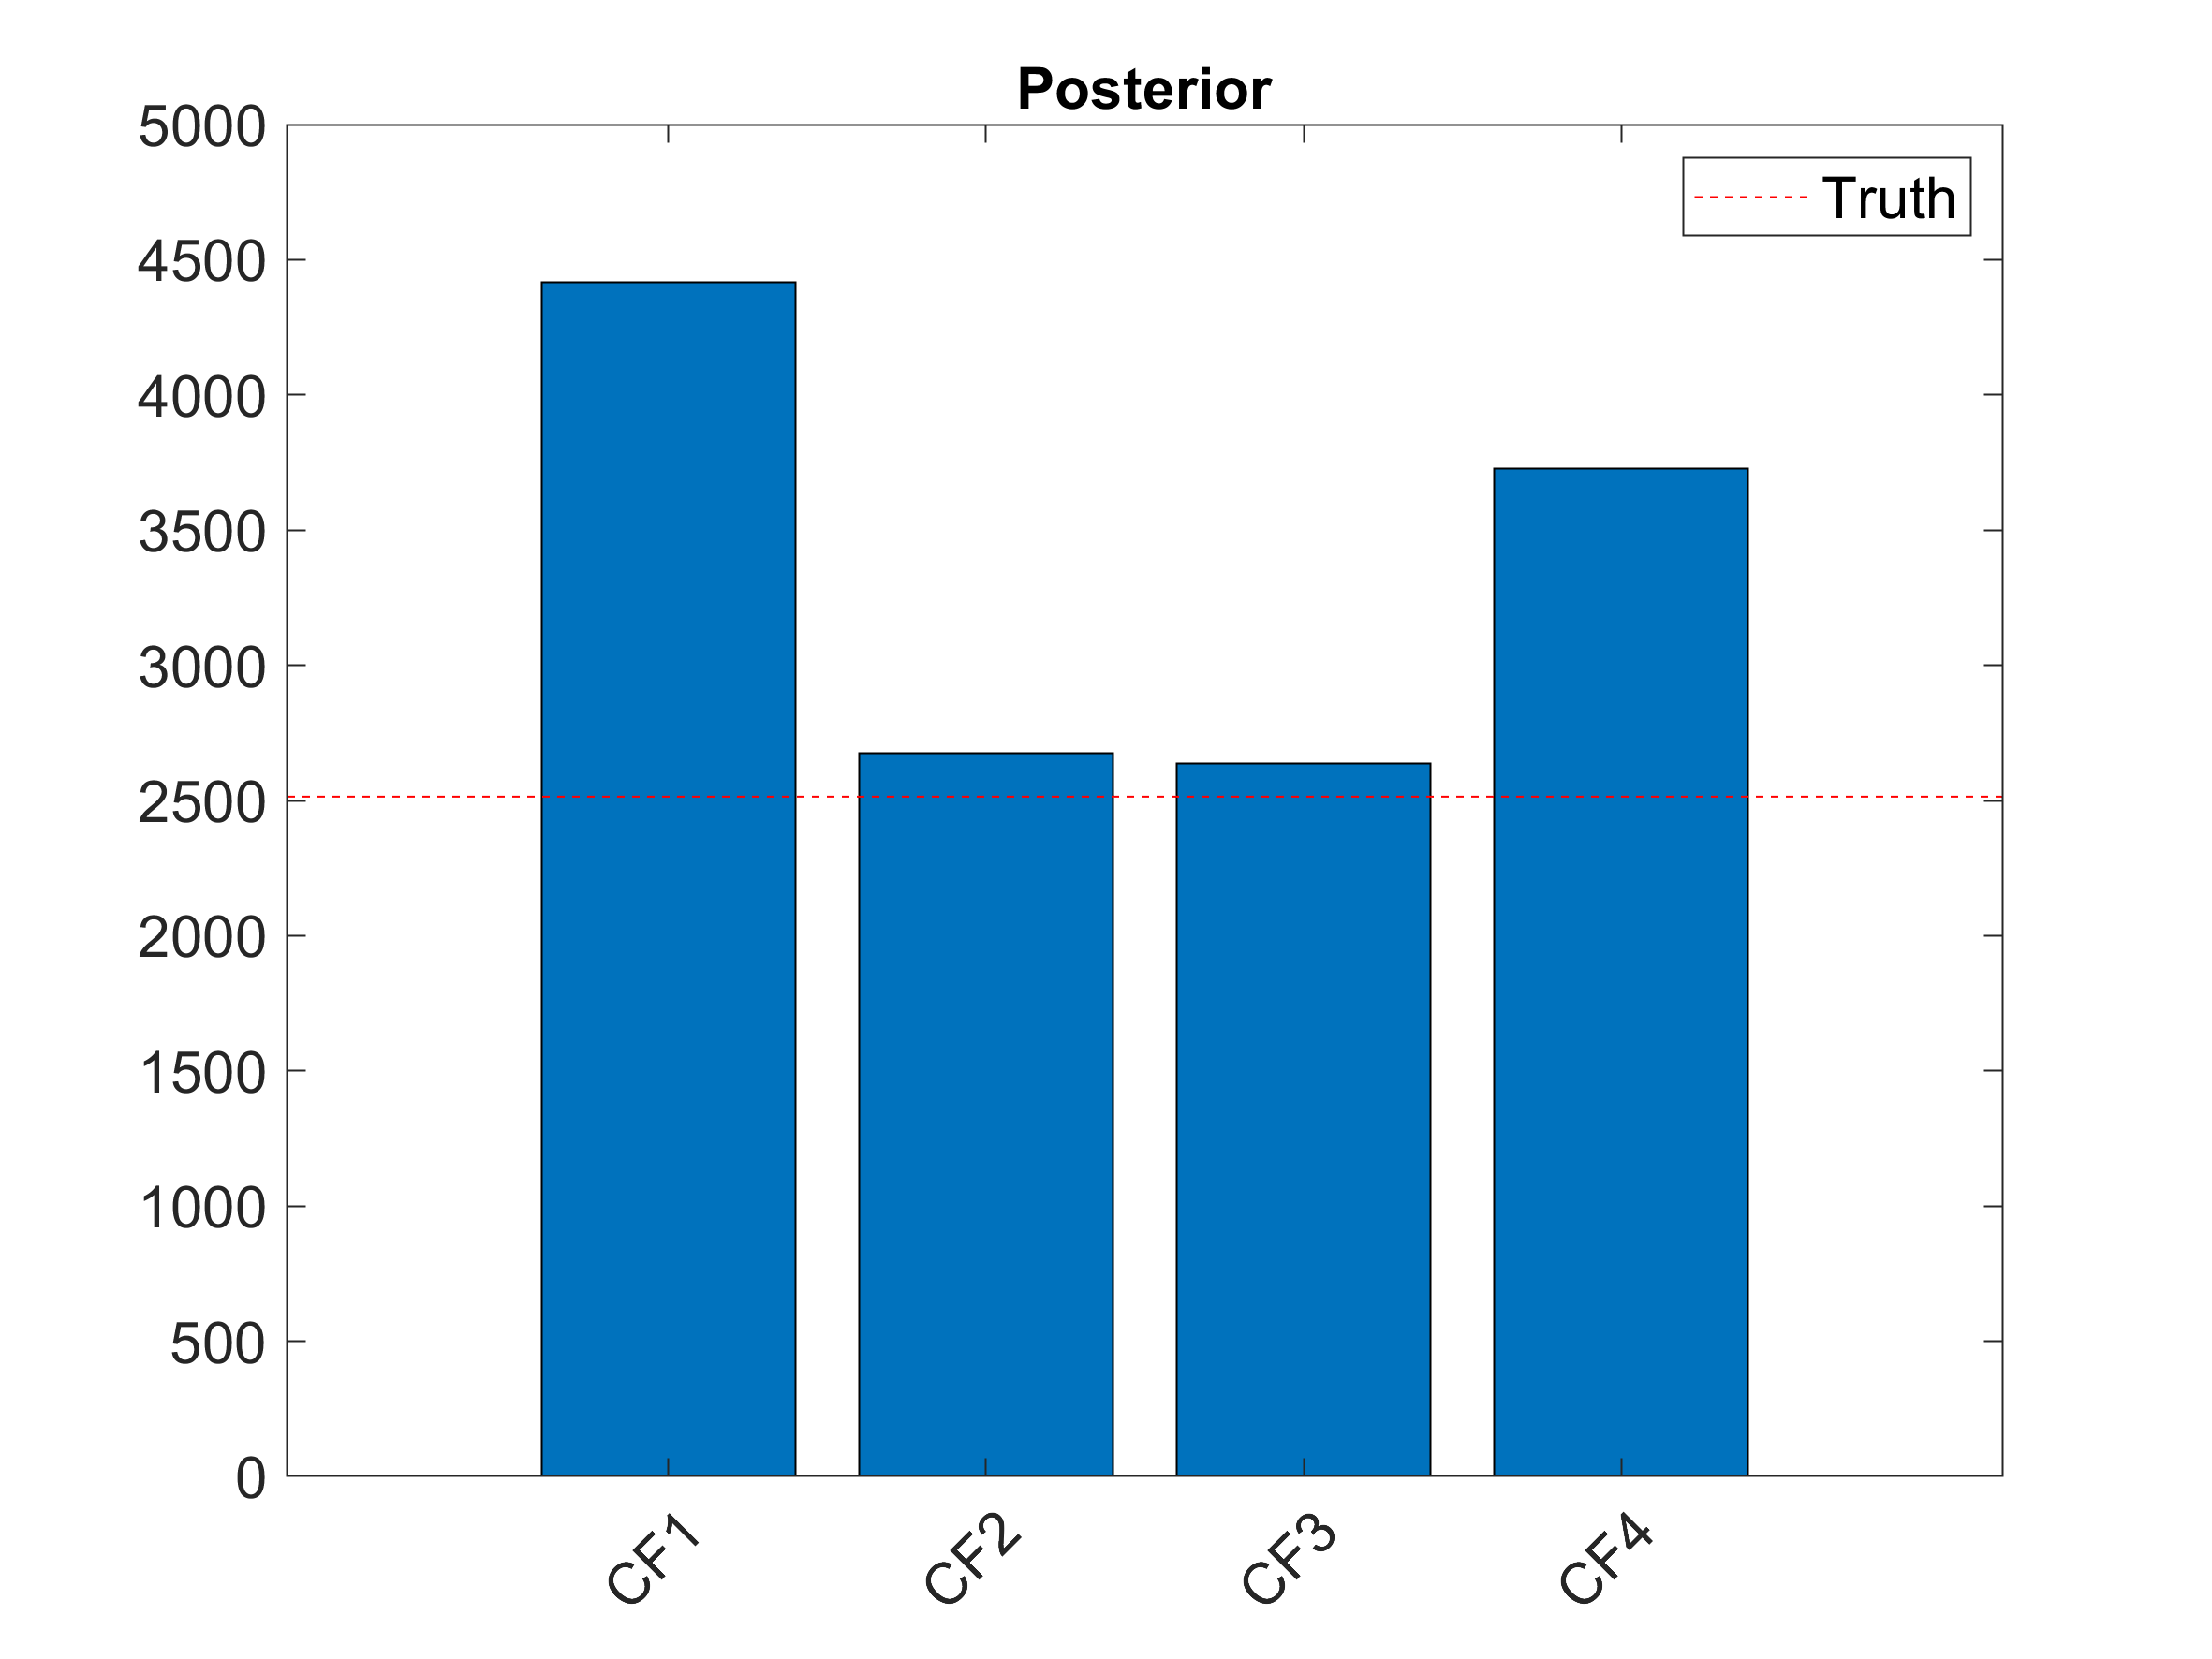
\includegraphics[width=0.8\textwidth]{./figures/res4.png}
%	\caption{Blob detection result. Blobs are detected where the local maximas are detected.}
%\end{figure}
%\begin{figure}[htbp]
%	\centering
%	\includegraphics[width=0.8\textwidth]{./figures/res5.png}
%	\caption{Blob detection result. Blobs are detected where the local maximas are detected.}
%\end{figure}
%\begin{figure}[htbp]
%	\centering
%	\includegraphics[width=0.8\textwidth]{./figures/res6.png}
%	\caption{Blob detection result. Blobs are detected where the local maximas are detected.}
%\end{figure}
%
%
%	\begin{figure}[htbp]
%		\centering
%		\includegraphics[width=0.9\textwidth]{./figures/sift_matching.png}
%		\caption{SIFT detection \& Matching Result.}
%	\end{figure}
%	\begin{figure}[htbp]
%	\centering
%	\includegraphics[width=0.9\textwidth]{./figures/projection.png}
%	\caption{Compute $2$D similarity transformation using \textsc{RANSAC}. After $s,\mathbf{R,t}$ is obtained, transform SIFT features in image $1$ to image $2$.}
%	\end{figure}
%	\begin{figure}[htbp]
%	\centering
%	\includegraphics[width=0.9\textwidth]{./figures/blob_projection.png}
%	\caption{Similar to previous image, but transform the blob detection results from image $1$ to image $2$. Red and blue circles denote the transformed and original detected blobs.}
%\end{figure}
%	\begin{figure}[htbp]
%	\centering
%	\includegraphics[width=0.9\textwidth]{./figures/hist.png}
%	\caption{Histogram of the absolute difference of diameters. The majortiy of the absolute differences are within $5$ pixels.}
%\end{figure}
%\begin{figure}
%	\centering
%	\includegraphics[width=0.9\textwidth]{./figures/a7.png}
%	\caption{Bacterial growth from movie frames. This is a snapshot of a single frame. See the complementary Gif for the animation.}
%	\includegraphics[width=0.7\textwidth]{./figures/a72}
%	\caption{Bacterial growth curve: assume one pixel equals to one bacteria.}
%\end{figure}
%\begin{figure}
%	\centering
%	\includegraphics[width=0.9\textwidth]{./figures/a7.png}
%	\caption{Bacterial growth from movie frames. This is a snapshot of a single frame. See the complementary Gif for the animation.}
%	\includegraphics[width=0.7\textwidth]{./figures/a72}
%	\caption{Bacterial growth curve: assume one pixel equals to one bacteria.}
%\end{figure}
%\begin{figure}
%	\centering
%	\includegraphics[width=0.9\textwidth]{./figures/a7.png}
%	\caption{Bacterial growth from movie frames. This is a snapshot of a single frame. See the complementary Gif for the animation.}
%	\includegraphics[width=0.7\textwidth]{./figures/a72}
%	\caption{Bacterial growth curve: assume one pixel equals to one bacteria.}
%\end{figure}
%	\begin{table}
%		\centering
%		\caption{{Quantitative result of Assignment $3$}}
%		\begin{tabular}{ccc}
%			\hline
%			\textbf{Image} &\textbf{Mean Diameters} & \textbf{Std of Diameters}  \\ \hline
%			\textbf{CT\_lab\_high\_res} & $8.9411$ &   $6.8761$   \\ \hline
%			\textbf{CT\_lab\_med\_res} & $7.6436$ &   $3.5724$  \\ \hline             
%			\hline
%		\end{tabular}
%		\label{tb:mittest}
%	\end{table}
	
	%\bibliography{PnPCites} 
	%\bibliographystyle{ieeetr}
	
\end{document}